%---PACKAGES----------------------------------------
\documentclass[a4paper,10pt]{article}

\usepackage{import}
\import{Packages/}{custom_packages.tex}
\import{Packages/}{custom_macros.tex}

\title{\textbf{Notes on Quiver Gauge Theories}}
\author{Louan Mol\\ \textit{Université Libre de Bruxelles}}
\date{}

% DOCUMENT -----------------------------

\begin{document}

\begin{titlepage}
    
    \maketitle

    \thispagestyle{empty}

    \vspace{2cm}

    \begin{abstract}
        In these notes, we present some basic ideas around the large topic of quiver gauge theories.  The goal is to reproduce and regroup the basics of quiver gauge theories. Note that this is a draft, it may contain a lot of typos, errors and imprecisions. It is only meant as a work support.
    \end{abstract}

    \vfill

    \hfill Last updated on \today.
    
\end{titlepage}
  
\pagebreak

\tableofcontents

\pagebreak

\nocite{*}

\section{Physical setup}

    \subsubsection*{Brane-world paradigm}

        We consider our world to be a slice in the ten-dimensional spacetime of type II superstring theory, i.e. the worldvolume of a D$3$-brane. More precisely, we consider a stack of $N$ D$3$-branes in order to have $\U(N)$ Chan-Paton factors resulting in a $\U(N)$ gauge group. To have D$3$-branes, we need to consider type IIB superstring theory. The spacetime is therefore not necessarily $\R^{1,9}$ but of the more general form
        \begin{equation*}
            M = \R^{1,3}\times M^{(6)}.\label{spacetimedecomp}
        \end{equation*}
        This is the so-called \emph{brane-world paradigm}. %In particular, we will be interested in type IIB string theory because of its self-duality under S-duality\marker.

    \subsubsection*{Supersymmetry and Calabi-Yau manifolds}
    
        Independently from string theory, we can ask for the wolrdvolume theory to be supersymmetric. We start from type IIB superstring theory which is $10$-dimensional and has $\mN=2$ supersymmetry so it possesses $32$ supercharges. As usual, they transform under the minimal spinor representation (MSR) of the bulk Lorentz group, here $\SO(1,9)$. In ten dimensions this representation is $8$-dimensional (complex) which is why there are $2(8+8)=32$ supercharges: $8$ transforming in the $8$-dimensional MSR and $8$ transforming in the $8$-dimensional conjugate MSR and whole thing times two since $\mN=2$. If we compactify type II string theory on $\R^{1,3}\times M^{(6)}$ where $M^{(6)}$ is any $6$-dimensional manifold, supersymmetry is broken. The reason for this is that the supercharges now have to transform under the MSR of $\SO(1,3)\times\H(M^{(6)})$\marker, where $\H(M^{(6)})$ is the holonomy group of $M^{6}$. Recall that a generic curved 6-dimensional manifold has $\O(6)$ holonomy and $\SO(6)$ if it is orientable. We only consider the later case. The supercharges must therefore transform under the MSR of $\SO(1,3)\times\SO(6)$. The MSR of $\SO(1,3)$ being $\boldsymbol{2}$ and the one of $\SO(6)$ being $\boldsymbol{4}$, we conclude that imposing the spacetime to have the form \eqref{spacetimedecomp} changes the representation under which the supercharges transform as follows:
        \begin{equation}
            \boldsymbol{8}\oplus\bar{\boldsymbol{8}}\to (\boldsymbol{2}_L,\boldsymbol{4})\oplus(\boldsymbol{2}_R,\bar{\boldsymbol{4}}).
        \end{equation}
        If we stop here, the residual supercharges might be ill-defined since making a tour around a loop in $M^{(6)}$ could result in anon-trivial rotation. To solve this problem, we need also to be more restrictive on the holonomy. In fact, it is precisely the holonomy of the transverse space that dictates the number of supersymmetries that are left. Let us now consider a four-dimensional field theory resulting from compactification of the transverse six-dimensional space. The number of supercharges that generate supersymmetries for this theory is the number of Killing spinor (covariantly constant spinor): each Killing spinor contracted with the local supersymmetry current generates a residual supersymmetry\marker. Now the link with holonomy: since $\SO(6)\cong\SU(4)$, minimal spinors can be viewed as having four complex component and as transforming under $\SU(4)$. Indeed, minimal spinors in six dimensions have four complex components. In order to have one covariantly conserved spinor, we look for the biggest subgroup of $\SU(4)$ that leaves a component of the spinor invariant. This is clearly $\{e\}\times\SU(3)\subset\SU(4)$ that acts trivially on the first component. The spinor $(1,0,0,0)$ is then covariantly conserved. Our transverse space must therefore have $\SU(3)$ holonomy such that the parallel transport of the spinor $(1,0,0,0)$ under any closed loop is a lower $\SU(3)$ rotation. We conclude that if the transverse Calabi-Yau has $\SU(3)$ holonomy, the worldvolume theory has $\mN=1$ supersymmetry. The same reasoning can be used to obtain that $\SU(2)$ holonomy implies $\mN=2$ supersymmetry.

        To conclude, preserving any degree of supersymmetry constrains the transverse space $M^{(6)}$ to be compact, complex, Kähler and to have $G\subset\SU(3)$ holonomy. Namely, $M^{(6)}$ must be a Calabi-Yau threefoldau manifolds are given in appendix \ref{sec:CY}.

    \subsubsection*{Non-compact transverse space}
    
        If we let the worldvolume of the D$3$-branes carry the requisite gauge theory while the bulk contains gravity, we can relax the compactness condition and study non-compact threefolds. In other words, $M^{(6)}$ is taken to be Calabi-Yau variety, instead of a Calabi-Yau manifold. A Calabi-Yau varitey is an affine variety that locally models a Calabi-Yau manifold, therefore allowing for singularities. 
        
        Using a non-compact transverse space can intuitively be understood as a Kaluza-Klein compactification where we take the size of the compact dimensions to infinity. The four-dimensional gravity coupling constant being inversely proportional to this quantity, there is no gravity in this limit. This makes the analysis much simpler and therefore also serves as an argument to ignore gravity in the worldvolume theory. Consequently, we will mostly ignore gravity and not care about the metric of the spacetime, see appendix \ref{app:spacetimegeom} for more details.

    \subsubsection*{Singular transverse space}

        The only smooth Calabi-Yau threefold is $\C^3$ so we are lead to consider singular Calabi-Yau varieties. We usually denote $S\equiv M^{(6)}$ to remind us of the singular aspect. String theory being a theory of extended objects, it is well-defined on such singularities. In a sense that will be clarified later, this singular structure of the geometry requires to ``project'' the theory. As a result, the gauge group $\U(N)$ will be broken down into products of smaller gauge groups. The simplest examples of singular Calabi-Yau varieties are Calabi-Yau orbifolds. We will mainly be interested these examples.
    
        From the point of view of the orbifold, the D$3$-brane is a point. Consequently, the D$3$-branes parametrize the transverse space. This is the first clue of the crucial relationship between the worldvolume theory and the Calabi-Yau singularity. Eventually, we will see that the classical vacuum of the gauge theory should be, in explicit coordinates, the defining equation of $S$. This is precisely the opposite of the projection manipulation we mentioned above: recovering the transverse space from the gauge theory. 
        
        Projecting and computing the classical vacua are therefore inverse operations with respect to each other. This suggest a bijection between the singular transverse space and the gauge theory: the former can be computed from the latter and vice-versa. This is called ``forward algorithm'' and ``inverse algorithm''. We will of course discuss this in more details.

    \subsubsection*{Mathematical formulation}

        Mathematically, this brane-world paradigm is the realization of branes as supports of vector bundles (sheaf). Gauge theories on branes are intimately related to algebraic constructions of stable bundles, i.e. holomorphic or algebraic vector bundles that are stable in the sense of geometric invariant theory. In particular, D-brane gauge theories manifest as a natural description of symplectic quotients and their resolutions in geometric invariant theory.

        To summarize in more mathematical terms, our D-branes, together with the stable vector bundle (sheaf) supported thereupon, resolves the transverse Calabi-Yau orbifold which is the vacuum for the gauge theory on the worldvolume as a GIT quotient \marker.

    \subsubsection*{Summary}

        We consider $N$ D$3$-branes in type IIB superstring theory carrying a $\U(N)$ gauge group. The transverse space $S$ is taken to be a non-compact singular Calabi-Yau variety.

\section{The simplest case: smooth transverse space}

    \subsection{Generalities}

        Let us start by considering the simplest configuration were the transverse Calabi-Yau space is non-singular, i.e. it is a proper smooth Calabi-Yau threefold. As mentioned above, the only smooth Calabi-Yau threefold is $S=\C^3$. In this case, the spacetime is simply flat space $\R^{1,9}=\R^{1,3}\times\R^6$ with a choice a complex structure on $\R^6$. From the $\U(N)$ Chan-Paton factors, the worldvolume theory inherits from a $\U(N)$ gauge group. Type IIB superstring theory is a ten-dimensional $\mN=2$ theory so it has $32$ supercharges. The presence of the branes breaks the Lorentz symmetry of $\R^{1,9}$ as
        \begin{equation}
            \SO(1,9)\to\SO(1,3)\times\SO(6),
        \end{equation}
        whereby breaking half of the supersymmetries, as we explained in the previous section. We are thus left with $16$ supercharges. In four dimensions, this corresponds to $\mN=4$. The worldvolume theory for $S=\C^3$ is therefore $D=4,\mN=4$ $\U(N)$ SCFT gauge theory. This worldvolume theory, obtained in the non-singular case $S=\C^3$, is called the \emph{parent theory}.

        Note that the D$3$-brane will warp the flat space metric to that of $AdS_5\times S^5$ and the bulk geometry is not strictly $\C^3$. However, as stated above, we are only concerned with the local gauge theory and not with gravitational back-reaction, therefore it suffices to consider $S$ as $\C^3$.

    \subsection{Matter content}

        As discussed in appendix \ref{sec:N4SCFT}, there is only one $D=4,\mN=4$ SCFT theory, up to a choice of gauge group $G$. In our case, $G=\U(N)$. The isometry group of the transverse space $\R^6$ is $\SO(6)\cong\SU(4)$. Since the scalar fields living on the branes are interpreted as its tranverse oscillations, $\SO(6)$ is a global symmetry of the field theory. These global symmetries of worldvolume theory lead to the R-symmetry group $\SU(4)_R$. The only $\mN=4$ supermutliplet can be rewritten in terms of $\mN=1$ supermultiplets as follows:
        \begin{equation}
            [\mN = 4 \text{ vector multiplet}] : V = (\lambda_\alpha, A_\mu, D) \oplus \Phi_A = (\phi^A,\psi^A_\alpha,F^A).
        \end{equation}
        with $A=1,2,3$. In other words, after removing the auxiliary fields $D$ and $F^A$, the matter content is
        \begin{itemize}
            \item a $\U(N)$ gauge field $A_\mu$ which transforms as a singlets under $\SU(4)_R$:
            \begin{align}
                \text{Gauge transformation} &: A_\mu\mapsto UA_\mu U^{-1}+U\p_\mu U^{-1},\qquad U\in\U(N)\label{eq:transfA1}\\
                \text{R-symmetry} &: A_\mu\mapsto A_\mu.\label{eq:transfA2}
            \end{align}
            Note that the usual term 
            \item $4$ Weyl fermions $\psi^{a}_\alpha\equiv(\lambda_\alpha,\psi^1_\alpha,\psi^2_\alpha,\psi^3_\alpha,)$ that transform under the adjoint of $\U(N)$ and are mixed together under the representation $\boldsymbol{4}$ of $\SU(4)_R$. This means that each fermion $\psi^a$ takes values in $\mathfrak{u}(N)$. We denote the components by $\psi^a_{IJ}$ ($I,J=1,\dots,N$). Explicitely:
            \begin{align}
                \text{Gauge transformation} &: \psi^a \mapsto U \psi^a U^\dagger ,\qquad U\in\U(N),\label{eq:transfpsi1}\\
                \text{R-symmetry} &: \psi^a\mapsto R\indices{^a_b}\psi^b,\qquad R\in\SU(4)_R.\label{eq:transfpsi2}
            \end{align}
            Note that this gives us $4N^2$ Weyl fermions in total.
            \item $3$ complex scalar fields $\phi^A$ transforming under the adjoint representation of $\U(N)$ and under the two-times anti-symmettric representation of $\SU(4)_R$. This means that each $\phi^A$ takes values in $\mathfrak{u}(N)$ and we denote the components by $\phi^A_{IJ}$. Recall that $\SU(4)\cong\SO(6)$ so the action of the R-symmetry can be seen as the $\boldsymbol{3}$ of $\SU(3)\subset\SU(4)_R$ acting on three complex scalars $\phi^A$ or equivalently as the $\boldsymbol{6}$ of $\SO(6)_R$ acting on $6$ real scalars $X^m$, the real and imaginary parts of the $\phi^A$. They are interpreted as the oscillations of the branes in the transverse space. Explicitely:
            \begin{align}
                \text{Gauge transformation} &: X^m \mapsto U X^m U^\dagger ,\qquad U\in\U(N),\label{eq:transfphi1}\\
                \text{R-symmetry} &: X^m \mapsto R\indices{^m_n}X^n,\qquad R\in\SO(6)_R.\label{eq:transfphi2}
            \end{align}
            Note that this gives $6N^2$ real scalars in total. They are the superpartners of the fermions\marker.
        \end{itemize}

        Note that the gauge group $\U(N)$ can also be seen as the group of isometries of the metric space $\C^N$, i.e. $\Hom(\C^N,C^N)$. From this point of view, the transformations \eqref{eq:transfA1}-\eqref{eq:transfphi2}can be summarized as
        \begin{align}
            A_\mu&\in\Hom(\C^N,\C^N),\label{eq:AHom}\\
            \psi&\in\boldsymbol{4}\otimes\Hom(\C^N,\C^N),\label{eq:psiHom}\\
            X&\in\boldsymbol{6}\otimes\Hom(\C^N,\C^N).\label{eq:phiHom}
        \end{align}

        \begin{result}
            If the transverse space is non-singular, the only possibility is $S=\C^3$. In this case, the worldvolume theory is therefore $D=4,\mN=4$ $\U(N)$ SCFT gauge theory. It is called the \emph{parent theory}.
        \end{result}

\part{Orbifold singularities}

\section{Singular transverse space: orbifold singularities}\label{sec:orbsing}

    When the transverse space is singular, the worldvolume theory corresponds to a specific projection of the parent theory that we found in the smooth case $S=\C^3$. We call it the \emph{daughter theory}. This projections depends on the type of singularity that one considers. The simplest case is the the case of orbifold singularity, i.e. when the transverse space is a quotient space with a non-free action.

    \subsection{Generalities}

        We now wish to pick a discrete group $\Gamma$ and which acts non-trivially on $\R^6$. There are several possibilities:
        \begin{itemize}
            \item $\Gamma\subset\SU(4)$ naturally acts on $\R^6$. This does not require a choice of complex structure. We get an $\mN=0$ theory.
            \item $\Gamma\subset\SU(3)$ naturally acts on $\C^3$, this also requires a choice of complex structure on $\R^6$. We get an $\mN=1$ theory.
            \item $\Gamma\subset\SU(2)$ naturally acts on the second factor of $\C\times\C^2$, so this requires a choice of complex structure on $\R^6$. We get an $\mN=2$ theory.
        \end{itemize}

        We are interested in supersymmetric theories so we take $\Gamma\subset\SU(3)$ with the action
        \begin{equation}
            \cdot:\left(
            \begin{array}{ccc}
                \Gamma\times\C^3 & \longrightarrow & \C^3 \\
                (\gamma,z) & \longmapsto & \gamma\cdot z
            \end{array}
            \right)
        \end{equation}
        is the representation of $\Gamma$ coming from the fundamental representation of $\SU(3)$, so $\cdot$ is just the matrix product. We can see that the origin is always a fixed point so this action is never free. Since $\C^3$ is a smooth manifold, this makes $\C^3/\Gamma$ an orbifold. Note this case naturally includes the case $\Gamma\subset\SU(2)$ too (as $\SU(2)\subset\SU(3)$), just not the case $\Gamma\in\SO(6)$. When $\Gamma\subset\SU(2\subset\SU(3)$, it acts trivially on one component so we write $S=\C\times\C^2/\Gamma$.

        If $\Gamma$ is a general finite group the condition that $\C^3/\Gamma$ is an Calabi-Yau orbifold means that there must exist a resolution of this orbifold such that the corresponding smooth space is Calabi-Yau, i.e. a crepant resolution. Existence of such a resolution constrains $\Gamma$ \marker, see appendix \ref{sec:CY}.

        If the transverse space is $S=\C^3/\Gamma$, the field theory must be projected to a theory which also invariant under $\Gamma$, seen as a subgroup of the R-symmetry group. The prescription is straihgt-forward: we can use the elements $\gamma\in\Gamma$ to project out that states that are not $\Gamma$-invariant. That is, if $\rho$ is an embedding of $\Gamma$ in the gauge group $\U(N)$, only the the fields such that
        \begin{align}
            \rho(\gamma) A_\mu \rho(\gamma)^{-1} &= A_\mu,\label{eq:proj1}\\
            R(\gamma)\rho(\gamma) \psi_{IJ} \rho(\gamma)^{-1} &= \psi_{IJ}\label{eq:proj2},\\
            R(\gamma)\rho(\gamma) X_{IJ} \rho(\gamma)^{-1} &= X_{IJ}\label{eq:proj3}
        \end{align}
        are kept in the spectrum, where $\rho$ is a unitary representation of $\Gamma$ on $\C^N$ and $R=\boldsymbol{4},\boldsymbol{6}$.
        Let us make two remarks:
        \begin{itemize}
            \item the term $U\p_\mu U^{-1}$ is absent from \ref{eq:proj1}. Indeed, $\Gamma$ is a finite group and the only smooth functions $x\mapsto\Gamma$ are the constant ones. Consequently, transformations of the gauge field under a finite subgroup of its gauge group cannot depend on $x$.
            \item the fields that transform non-trivially under R-symmetry also have an extra induced action of $\Gamma$, in agreement with \eqref{eq:AHom}-\eqref{eq:phiHom}. The R-symmetry untouched by $\Gamma$ will be the resulting R-symmetry of daughter theory.
        \end{itemize}

    \subsection{Representation theory realization}

        Let $\{(\rho_i,V_i)\}_{i\in I}$ be a complete set of irreducible representations of $\Gamma$. Since $\Gamma$ is finite, it is particular compact and those representation can be taken to be unitary. Moreover, $i$ takes a finite number of values. Let us consider a representation of $\Gamma$ on $\C^N$, we denote it $(\rho,\C^N)$ and also take it to be unitary. In that case, $\rho(\gamma)\in\U(N)$. This is what we mean by ``the embedding of $\Gamma$ in $\U(N)$''. The adjoint representation of $\U(N)$ defined as\footnote{this is well-defined since for all $\omega\in\mathfrak{u}(N)$ and $U\in\U(N)$, $U\omega U^{-1}\in\mathfrak{u}(N)$.}
        \begin{equation}
            \Ad:\left(
            \begin{array}{ccc}
                \U(n) & \longrightarrow & \GL(\mathfrak{u}(N)) \\
                U & \longmapsto & \Ad_U
            \end{array}
            \right),\qquad
            \Ad_U:\left(
            \begin{array}{ccc}
                \mathfrak{u}(N) & \longrightarrow & \mathfrak{u}(N) \\
                \omega & \longmapsto & \Ad_U(\omega)\equiv U\omega U^{-1}
            \end{array}
            \right),
        \end{equation}
        now allows us to act with $\Gamma$ on $\mathfrak{u}(N)$. We use this representation in the expression \eqref{eq:proj1}-\eqref{eq:proj3}. More formally, these relations can be rewritten as
        \begin{align}
            \Ad_{\rho(\gamma)}A_\mu  &= A_\mu,\\
            R(\gamma)\Ad_{\rho(\gamma)}\psi_{IJ}  &= \psi_{IJ},\\
            R(\gamma)\Ad_{\rho(\gamma)}X_{IJ} &= X_{IJ}
        \end{align}
        

        We can decompose $(\rho,\C^N)$ as follows:
        \begin{align}
            (\rho,\C^N) &= \bigoplus_{i\in I}~(\rho_i,V_i)^{N_i} \\
            &= \bigoplus_{i\in I}~(\boldsymbol{1}^{N_i}\otimes\rho_i,\C^{N_i}\otimes V_i) \label{eq:decomp:line2}
        \end{align}
        were $N_i$ are integer multiplicities ($(\rho_i,V_i)^{N_i}\equiv(\rho_i,V_i)^{\oplus N_i}$) and $\boldsymbol{1}$ is the trivial representation, so $\Gamma$ acts trivially on the $\C^{N_i}$. We have $\sum_iN_i\dim(\rho_i)=N$. The rewritting \eqref{eq:decomp:line2} will be useful later on.
        
        After the projection, the resulting gauge group is given by the $\Gamma$-invariant part of the gauge group, that is $\Hom(\C^N,\C^N)^\Gamma$. We use the superscript $\Gamma$ to indicate that we only keep the trivial representations in the decomposition, that is, we only keep that subspaces that transform trivially. First, we can see that by Schur's lemma \marker
        \begin{equation}
            (V_i\otimes V^*_j)^\Gamma=\delta_{ij}
        \end{equation}
        
        Now since $\Hom(\C^N,\C^N)\cong\C^N\otimes(\C^N)^*$, we get
        \begin{align}
            \Hom(\C^N,\C^N)^\Gamma &= (\C^N\otimes(\C^N)^*)^\Gamma\\
            &= \bigoplus_{i,j\in I} \left((\C^{N_i}\otimes V_i)\otimes(\C^{N_j}\otimes V_j)^*\right)^\Gamma\\
            &= \bigoplus_{i,j\in I} \left(\C^{N_i}\otimes(\C^{N_j})^*\otimes V_i\otimes V^*_j\right)^\Gamma\\
            &= \bigoplus_{i,j\in I} \left(\C^{N_i}\otimes(\C^{N_j})^*\right)^\Gamma\otimes\left(V_i\otimes V^*_j\right)^\Gamma\\
            &= \bigoplus_{i\in I}\C^{N_i}\otimes(\C^{N_i})^*
        \end{align}
        so the daughter gauge group is
        \begin{equation}
            G_{\text{proj}} = \bigotimes_{i\in I}\U(N_i).
        \end{equation}
        Now it turns out that in the low energy effective field theory the $\U(1)$ factor of every $\U(N_i)$ decouples \marker so the resulting gauge group is in fact
        \begin{equation}
            G_{\text{proj}} = \bigotimes_{i\in I}\SU(N_i).
        \end{equation}

        For the matter fields, the reasoning is similar but we now have to take into account the R-symmetry. Let $\boldsymbol{4}\equiv(\rho_{\boldsymbol{4}},V_{\boldsymbol{4}})$ be the fundamental representation of $\SU(4)_R$ and $\boldsymbol{6}\equiv(\rho_{\boldsymbol{6}},V_{\boldsymbol{6}})$ be the fundamental representation of $\SO(6)_R$. Wish to compute $(V_\mR\otimes\Hom(\C^N,\C^N))^\Gamma$ with $\mR=\boldsymbol{4},\boldsymbol{6}$:
        \begin{align}
            (V_\mR\otimes\Hom(\C^N,\C^N))^\Gamma &= \bigoplus_{i,j\in I} \left(V_\mR\otimes (\C^{N_i}\otimes V_i)\otimes(\C^{N_j}\otimes V_j)^*\right)^\Gamma\\
            &= \bigoplus_{i,j\in I} \left(V_\mR\otimes\C^{N_i}\otimes(\C^{N_j})^*\right)^\Gamma\otimes\left(V_i\otimes V^*_j\right)^\Gamma\\
            &= \bigoplus_{i,j\in I}a^\mR_{ij}\left(\C^{N_i}\otimes(\C^{N_j})^*\right)\label{eq:resdecomp}
        \end{align}
        with
        \begin{equation}
            (\rho_\mR,V_\mR)\otimes(\rho_i,V_i)=\bigoplus_{j\in I}a^\mR_{ij}(\rho_j,V_j).\label{eq:defaij}
        \end{equation}
        This expression makes sense because $(\rho_\mR,V_\mR)$ is a representation of $\SU(4)$ so it is in particular a representation of $\SU(3)$ and therefore also in particular a representation of $\Gamma$.

        Using the orthogonality of characters of irreducible non-equivalent representations, we obtain the explicit expression of the coefficient $a^\mR_{ij}$:
        \begin{equation}
            a^\mR_{ij} = \frac{1}{\abs{\Gamma}}\sum^r_{\gamma=1} r_\gamma\chi^\mR(\gamma)\chi^i(\gamma)\chi^j(\gamma)^*
        \end{equation}
        where $r_\gamma$ is the order of the conjugacy class containing $\gamma$ and $\chi^i$ is the character of $\rho_i$.

        In the end, we can see that:
        \begin{result}
            In the daughter theory, the matter fields become a total of $a^{\boldsymbol{4}}_{ij}$ bi-fundamental fermions and $a^{\boldsymbol{6}}_{ij}$ bi-fundamental bosons transforming as the $(\boldsymbol{\textbf{N}_i},\boldsymbol{\bar{\textbf{N}}_j})$ of $\SU(N_i)\times\SU(N_j)$ under the products of gauge groups.
        \end{result}

    \subsection{Field content, quivers and McKay graphs}

        A convenient way the represent the matter content of a daughter theory is to use \emph{quiver diagrams}. A quiver is a finite oriented graph such that each node $i$ represents a gauge factor $\SU(N_i)$ and each arrow $i\to j$ represents a bi-fundamental field transforming under $(\boldsymbol{\textbf{N}_i},\boldsymbol{\bar{\textbf{N}}_j})$. The \emph{adjacency matrix} $A$ of the graph is a $k\times k$ with $k$ being the number of nodes (gauge factors) whose elements $A_{ij}$ are the number of arrows (bi-fundamental fields) from $i$ to $j$. In other words, from \eqref{eq:resdecomp}, the adjacency matrix of the fermions has elements $A_{ij}=a^{\boldsymbol{4}}_{ij}$ and the one of the scalars has elements $A_{ij}=a^{\boldsymbol{6}}_{ij}$.

        On the other hand, given finite group $\Gamma$, a representation $(\rho_W,W)$ and a complete set of irreducible representations $\{(\rho_i,V_i)\}_{i\in I}$ of the latter, one can construct a McKay graph (or quiver) as follows:
        \begin{enumerate}
            \item Draw a vertex for every representation $(\rho_i,V_i)$.
            \item For every representation $(\rho_i,V_i)$, compute the decomposition
            \begin{equation*}
                (\rho_W,V_W)\otimes(\rho_i,V_i)=\bigoplus_j (\rho_j,V_j)^{\oplus n_{ij}}
            \end{equation*}
            where $n_{ij}$ is the multiplicity of $(\rho_j,V_j)$ in the decomposition of $(\rho_W,V_W)\otimes(\rho_i,V_i)$.
            \item For every $n_{ij}>0$, draw $n_{ij}$ arrows from the vertex of $(\rho_i,V_i)$ to the one of $(\rho_j,V_j)$.
        \end{enumerate}
        When $\Gamma\subset\SU(2)$ and that $(\rho_W,W)$ is its defining representation, the McKay graphs are in one-to-one correspondence with the extended Dynkin diagrams of the simply laced Lie algebras. This is the classical McKay correspondence, see appendix \ref{app:McKay}.
        
        From \eqref{eq:defaij} we see that $n_{ij}=a^{\mR}_{ij}$, i.e. the matter quivers that we defined previously are exactly the McKay graph associated to the matter representation in question. Put differently, the matter content of the daughter theory is encapsulated in the McKay graphs of $\Gamma$ and with respect to $\mR$ with $\mR=\bs{4}$ for spinors and $\mR=\bs{6}$ for scalars. This very important point allows us to use known results on McKay graphs such as the McKay correspondence for example.


    \subsection{A simple example: $S=\C^3/\Z_3$}\label{sec:C3Z3}

        We illustrate the previous discussion by the simple case where $\Gamma=\Z_3$ acts on $\C^2$ as
        \begin{equation}
            \begin{bmatrix}
                z_1\\z_2\\z_3
            \end{bmatrix}\mapsto
            \begin{bmatrix}
                \zeta_3 & 0 & 0 \\
                0 & \zeta_3 & 0 \\
                0 & 0 & \zeta_3
            \end{bmatrix}
            \begin{bmatrix}
                z_1\\z_2\\z_3
            \end{bmatrix}
        \end{equation}
        i.e. the transverse space is the orbifold $\C^3/\Z_3$. This simple example is a good first approach in which we will to explain in details each step so that we can go faster afterwards.

        \subsubsection{Projection}

            Let us consider a representation $(\rho,\C^N)$ of $\Z_3$. A complete set of irreducible representations of $\Z_3$ is given by $\{(\rho_k,V_k)\}_{k=0,1,2}$ with $V_k=\C$ and
            \begin{equation}
                \rho_i(g)=\zeta^k_3
            \end{equation}
            where $g$ is the generator of $\Z_3$. The representation $(\rho,V)$ can be decomposed as
            \begin{equation}
                (\rho,V)=\bigoplus^{2}_{i=0}N_i(\rho_i,V_i).
            \end{equation}
            In other words, it is equivalent to the representation
            \begin{equation}
                \rho(g)=
                \begin{bmatrix}
                    1 & & & & \cdots & & & & & 0 \\
                    & \ddots & & & & & & & & \\
                    & & 1 & & & & & & & \\
                    & & & \zeta_3 & & & & & & \\
                    \vdots & & & & \ddots & & & & & \vdots \\
                    & & & & & \zeta_3 & & & & \\
                    & & & & & & & \zeta^2_3 & & \\
                    & & & & & & & & \ddots & \\
                    0 & & & & \cdots & & & & & \zeta^2_3 \\
                \end{bmatrix}
                \hspace{-0.2cm}
                \begin{tabular}{l}
                $\left.\lefteqn{\phantom{
                    \begin{matrix}
                        a_0\\ \ddots\\ a_0\ 
                    \end{matrix} 
                }}\right\}N_0$\\
                $\left.\lefteqn{\phantom{
                    \begin{matrix}
                        a_0\\ \ddots\\ a_0\ 
                    \end{matrix} 
                }}\right\}N_1$\\
                $\left.\lefteqn{\phantom{
                    \begin{matrix}
                        b_0\\ \ddots\\ b_0\ 
                    \end{matrix}
                }} \right\}N_2$
                \end{tabular}.\label{eq:reprrhoZn}
            \end{equation}
            Since $\dim\rho_i=1$, we have
            \begin{equation}
                N_0+N_1+N_2=N.\label{eq:sumNiZ3}
            \end{equation} 
            
            The gauge field configurations that are left invariant under the action of $\Z_n$ are therefore the ones that satisfy
            \begin{equation}
                \rho(g)A_\mu\rho(g)^{-1}=A_\mu.\label{eq:AinvZ3}
            \end{equation}
            We actually want this relation to be true for any element of $\Z_n$ but in this case it is invariant under any element of $\Z_n$ if and only if it is invariant under the generator $g$ of $\Z_3$, so we only need to impose \eqref{eq:AinvZ3}. The constrained is easily solved by using the bi-index notation $A_{\mu;i\alpha_i,j\beta_j}$ ($i,j=0,1,2,\alpha_i,\beta_i=1,\dots,N_i$) for the component of the gauge fields. From \eqref{eq:reprrhoZn}, we can see that
            \begin{equation}
                A_{\mu;i\alpha_i,i\beta_j}\mapsto \rho_i(g)A_{\mu;i\alpha_i,j\beta_j}\rho_j(g)^{-1}=\zeta^{i-j}_nA_{\mu;i\alpha_i,j\beta_j}.
            \end{equation}
            thus only the configurations with $A_{\mu;i\alpha_i,j\beta_j}=0$ if $i\neq j$ are invariant. The gauge field has therefore a block diagonal form:
            \begin{equation}
                A_\mu=
                \begin{bmatrix}
                    A_{\mu;00} & & \\
                    & A_{\mu;11} & \\
                    & & & A_{\mu;2,2}
                \end{bmatrix}
            \end{equation}
            with $A_{\mu;ij}\equiv (A_{\mu;i\alpha_i,j\beta_j})_{\alpha_i=0,\dots,N_i,\beta_j=0,\dots,N_j}$. The block $A_{ii}$ transforms under $\Z_3$ under $(\rho_i,V_i)^{N_i}$.
            Consequently, the gauge group is now broken to
            \begin{equation}
                G_{\text{proj}}=\U(N_0)\times\U(N_1)\times\U(N_1),
            \end{equation}
            the biggest subgroup of $\U(N)$ that preserves those form of configurations.
            
            Let us study the scalars. $\Z_3$ acts on the three complex scalars through
            \begin{equation}
                R(g)= \rho^{\oplus 3}_1(g) = \zeta_3\mathbbm{1}_3 =
                \begin{bmatrix}
                    \zeta_3 & 0 & 0 \\
                    0 & \zeta_3 & 0 \\
                    0 & 0 & \zeta_3
                \end{bmatrix}
            \end{equation}
            or, equivalently, on the real scalars as $R(g)=\zeta_3\mathbbm{1}_6$. According to \eqref{eq:transfphi1}-\eqref{eq:transfphi2}, the scalar field configurations that are left invariant satisfy
            \begin{equation}
                R(g)\indices{^m_n}\rho(g)X^n\rho(g)^{-1}=X^m
            \end{equation}
            for all $g\in\Z_n$. Using the bi-index notations, this becomes
            \begin{align}
                X^m_{i\alpha_i,j\beta_j}\mapsto  \zeta_n\delta\indices{^m_n}\rho_i(g) X^n_{i\alpha_i,j\beta_j}\rho_j(g)^{-1} = \zeta^{i-j+1}_3X^m_{i\alpha_i,j\beta_j}\\
                \bar{X}^m_{i\alpha_i,j\beta_j}\mapsto  \zeta^{-1}_3\delta\indices{^m_n}\rho_i(g) \bar{X}^n_{i\alpha_i,j\beta_j}\rho_j(g)^{-1} = \zeta^{i-j-1}_3\bar{X}^m_{i\alpha_i,j\beta_j}
            \end{align}
            thus only the configurations with $X^n_{i\alpha_i,j\beta_j}=0$ if $i-j+1\neq0$ are left invariant and only the configurations with $\bar{X}^n_{i\alpha_i,j\beta_j}=0$ if $i-j-1\neq0$ are left invariant. The scalar fields $X$ have a block off-diagonal form:
            \begin{equation}
                X^m=
                \begin{bmatrix}
                    0 & X^m_{01} & 0 \\
                    0 & 0 & X^m_{12} \\
                    X^m_{21} & & 0
                \end{bmatrix},\qquad
                \bar{X}^m=
                \begin{bmatrix}
                    0 & 0 & \bar{X}^m_{02} \\
                    \bar{X}^m_{10} & 0 & 0 \\
                    0 & \bar{X}^m_{21} & 0
                \end{bmatrix}
            \end{equation}
            with the block notations
            \begin{align*}
                X^m_{ij}&\equiv (X^m_{i\alpha_i,j\beta_j})_{\alpha_i=0,\dots,N_i,\beta_j=0,\dots,N_j}\\
                \bar{X}^m_{ij}&\equiv (\bar{X}^m_{i\alpha_i,j\beta_j})_{\alpha_i=0,\dots,N_i,\beta_j=0,\dots,N_j}.
            \end{align*}
            The block $X^m_{ij}$ is an $N_i\times N_j$ block and transforms under the representation $(\boldsymbol{\textbf{N}_i},\boldsymbol{\bar{\textbf{N}}_j})$ of $\U(N_i)\times\U(N_j)$:
            \begin{align}
                X^m_{i,i+1} &\in \boldsymbol{\textbf{N}_{i+1}}\otimes\boldsymbol{\bar{\textbf{N}}_i} \cong \Hom(V_{i+1},V_i),\\
                \bar{X}^m_{i+1,i} &\in \boldsymbol{\textbf{N}_{i}}\otimes\boldsymbol{\bar{\textbf{N}}_{i+1}} \cong \Hom(V_{i},V_{i+1}).
            \end{align}
            Let us make an important observation: the form of the scalar fields are the same for every $m=0,\dots,5$. This can be traced back to the fact that $R(g)=\zeta_3\mathbbm{1}_6$ so the R-symmetry action of $\Z_n$ is the same for all $m$.

            Let us now study the four Weyl fermions $\psi^a$.\marker

        \subsubsection{Quiver}

            We can draw the quiver of this daughter theory. We have three types of bi-fundamental scalar fields:
            \begin{equation}
                X^m_{01}\in(\boldsymbol{\textbf{N}_{1}},\boldsymbol{\bar{\textbf{N}}_0}),\quad
                X^m_{12}\in(\boldsymbol{\textbf{N}_{2}},\boldsymbol{\bar{\textbf{N}}_1}),\quad
                X^m_{20}\in(\boldsymbol{\textbf{N}_{0}},\boldsymbol{\bar{\textbf{N}}_2}).
            \end{equation}
            In each representation bi-fundamental representation there are six real scalars, i.e. 3 complex scalars. They are each represented by an arrow between the right representations, see fig. \ref{fig:Z3quiver}.
            \begin{figure}[H]
                \centering
                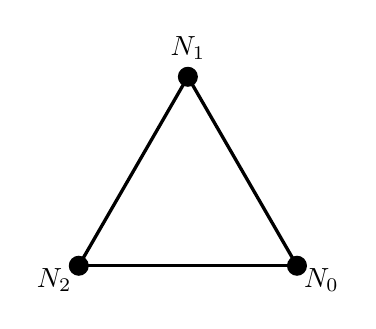
\begin{tikzpicture}[scale=0.8]
                    \foreach \n in {0,...,2}{
                        \draw[very thick] ({-120*\n-30}:2)--({-120*(\n+1)-30}:2) node[midway,sloped,allow upside down]{$\blacktriangleright\blacktriangleright\blacktriangleright$};
                        \draw[fill=black] ({-120*\n-30}:2) circle[radius=0.15];
                    }
                    \draw (-30:2.45) node{$N_0$};
                    \draw (90:2.45) node{$N_1$};
                    \draw (210:2.45) node{$N_2$};
                \end{tikzpicture}
                \caption{Quiver of the $\C^3/\Z_3$ daughter theory.}
                \label{fig:Z3quiver}
            \end{figure}
            The adjacency matrix of this quiver is
            \begin{equation}
                A=
                \begin{bmatrix}
                    0 & 3 & 0 \\
                    0 & 0 & 3 \\
                    3 & 0 & 0
                \end{bmatrix}
            \end{equation}
            which is coherent with the fact that the coefficients of the McKay decomposition of $\rho_1\oplus\rho_1\oplus\rho_1$ are
            \begin{align}
                \begin{split}
                    n_{00} &= 0,\quad n_{01} = 3\qquad n_{02}=0,\\
                    n_{10} &= 0,\quad n_{11} = 0,\qquad n_{12}=3,\\
                    n_{20} &= 3,\quad n_{21} = 0,\qquad n_{22}=0.
                \end{split}
            \end{align}

        \subsubsection{Gauge anomaly cancellation}
        
            Finally, let us discuss the gauge anomaly cancellation. Our fields transform under the adjoint representation of $\SU(N)$, under the fundamentals of $\SU(N_i)$ and under the anti-fundamentals of $\SU(N_i)$. The adjoint representation being reel, it is self-conjugate and therefore does not contribute to the anomaly. Fundamentals of $\SU(N_i)$ have a $+1$ contribution to the anomaly and anti-fundamentals of $\SU(N_i)$ have a $-1$ contribution to the anomaly. Anomaly cancellation therefore imposes that the contribution of the fundamental and of the anti-fundamental of $\SU(N_i)$ cancel each other for each $i=0,1,2$, see appendix \eqref{sec:anomalies}. The bi-fundamental representation $(\boldsymbol{\textbf{N}_i},\boldsymbol{\bar{\textbf{N}}_j})$ counts as $N_j$ fundamentals of $\SU(N_i)$ and as $N_i$ anti-fundamentals $\SU(N_j)$. We get the three following conditions:
            \begin{align}
                \SU(N_0) &: N_2-N_1 = 0,\\
                \SU(N_1) &: N_0-N_2 = 0,\\
                \SU(N_2) &: N_1-N_0 = 0.
            \end{align}
            which immediately imply
            \begin{equation}
                N_0=N_1=N_2.
            \end{equation}
            From \eqref{eq:sumNiZ3}, we get that $N_0=N_1=N_2=N/3$, meaning that that the daughter theory has quantum gauge symmetry if and only if the parent theory with has gauge group $\SU(N)$ where $N$ is a multiple of $3$. Or, in other words, if the number of D-branes is a multiple of $3$.

    \subsection{$(p+1)$-dimensional quiver gauge theories}

        Let us mention that we can generalize our initial brane-world paradigm and consider D$p$-branes in type II string theory (type IIA if $p$ is even and type IIB if $p$ is odd) instead of just D$3$-branes. The spacetime is then of the form
        \begin{equation}
            M = \R^{1,p}\times\R^{9-p}/\Gamma
        \end{equation}
        where $\Gamma$ is a discrete subgroup of $\Spin(9-p)$. If $\Gamma$ is a subgroup of a special holonomy group, we recover a somewhat generalized version of the paradigm that we discussed above. In this case the transverse space is a Calabi-Yau orbifold and some degree of supersymmetry is preserved. Note that the fermionic and bosonic quivers that coincides. If $\Gamma$ is not a subgroup of a special holonomy group, then the $(p+1)$-dimensional quiver gauge theory that we obtain in the low-energy limit is not supersymmetric. We then have different quivers for the fermions and the bosons, although with the same vertices, by definition.

        Recall that the fraction of supercharges that is preserved by compactifying on a Calabi-Yau $n$-fold (with $\SU(n)$ holonomy) is $2^{1-n}$. Starting from the $\mN=2$ 10-dimensional type IIB string theory with 32 supercharges, this means that
        \begin{itemize}
            \item if we compactify on a $1$-fold, we get $32$ supercharges in $8$ dimensions so $\mN=2$,
            \item if we compactify on a $2$-fold, we get $16$ supercharges in $6$ dimensions so $\mN=2$,
            \item if we compactify on a $3$-fold, we get $8$ supercharges in $4$ dimensions so $\mN=2$,
            \item is we compactify on a $4$-fold, we get $4$ supercharges in $2$ dimensions so $\mN=4$.
        \end{itemize}

        We will however mostly mostly consider $4$-dimensional quiver gauge theories, i.e. living on D$3$-branes.
    

\section{$\mN=2$ daughter theories}\label{sec:N2QGT}

    %Let us consider that $\Gamma$ is a finite subgroup of $\SU(2)\subset\SU(3)$. It naturally acts on $\C^3$ trough its fundamental representation $\bs{2}$ as $\bs{1}\oplus\bs{2}$ (only acts on 2 coordinates).

    \subsection{$S=\C\times\C^2/\Z_n$}

        We consider a representation $(\rho,\C^N)$ of $\Z_n$. We decompose it on the set of irreducible representations of $\Z_n$ as
        \begin{equation}
            (\rho,V)=\bigoplus^{n-1}_{i=0}N_i(\rho_i,V_i).
        \end{equation}
        In other words, it is equivalent to the representation
        \begin{equation}
            \rho(g)=
            \begin{bmatrix}
                1 & & & \cdots & & & 0 \\
                & \ddots & & & & & \\
                & & 1 & & & &  \\
                \vdots & & & \ddots & & & \vdots \\
                & & & & \zeta^{n-1}_n & & \\
                & & & & & \ddots & \\
                0 & & & \cdots & & & \zeta^{n-1}_n 
            \end{bmatrix}
            \hspace{-0.2cm}
            \begin{tabular}{l}
            $\left.\lefteqn{\phantom{
                \begin{matrix}
                    a_0\\ \ddots\\ a_0\ 
                \end{matrix} 
            }}\right\}N_0$\\
            \vdots \\
            $\left.\lefteqn{\phantom{
                \begin{matrix}
                    b_0\\ \ddots\\ b_0\ 
                \end{matrix}
            }} \right\}N_{n-1}$
            \end{tabular}.\label{eq:reprrhoZn}
        \end{equation}
        Since $\dim\rho_i=1$, $\sum_i N_i=N$. 

        The gauge field configurations that are left invariant under the action of $\Z_n$ are therefore the ones that satisfy
        \begin{equation}
            \rho(g)A_\mu\rho(g)^{-1}=A_\mu.
        \end{equation}
        The constrained is easily solved by using the bi-index notation:
        \begin{equation}
            A_{\mu;i\alpha_i,i\beta_j}\mapsto \rho_i(g)A_{\mu;i\alpha_i,j\beta_j}\rho_j(g)^{-1}=\zeta^{i-j}_nA_{\mu;i\alpha_i,j\beta_j}.
        \end{equation}
        thus only the configurations with $A_{\mu;i\alpha_i,j\beta_j}=0$ if $i\neq j$ are invariant. The gauge field has therefore a block diagonal form:
        \begin{equation}
            A_\mu=
            \begin{bmatrix}
                A_{\mu;00} & & & \\
                & A_{\mu;11} & & \\
                & & \ddots & \\
                & & & A_{\mu;n-1,n-1}
            \end{bmatrix}
        \end{equation}
        with $A_{\mu;ij}\equiv (A_{\mu;i\alpha_i,j\beta_j})_{\alpha_i=0,\dots,N_i,\beta_j=0,\dots,N_j}$. The block $A_{ii}$ transforms under $\Z_n$ as $(\rho_i,V_i)^{N_i}$. For now it is only a simple generalization of the case $\C^3/\Z_3$. This makes sense: projection of the gauge field only depends the discrete group $\Gamma$, not on the way it acts on $\C^3$ because it does not transform under R-symmetry.
        
        The gauge group is now broken to
        \begin{equation}
            G_{\text{proj}}=\prod^{n-1}_{i=0}~\U(N_i).
        \end{equation}

        Now for the scalar fields. The action of $\Z_n$ that we consider leaves the first component of $\C^3$ untouched so we take the action $\boldsymbol{1}\oplus\boldsymbol{2}$ where $\boldsymbol{2}$ is the usual action of $\Z_n$ on $\C^2$. In other words, 
        \begin{equation}
            R(g)=
            \begin{bmatrix}
                1 & 0 & 0 \\
                0 & \zeta_n & 0 \\
                0 & 0 & \zeta^{-1}_n
            \end{bmatrix}.
        \end{equation}
        Or, equivalently, $R(g)\indices{^m_n}=\delta\indices{^m_n}A_n$ with $A_m=(1,1,\zeta_n,\zeta_n,\zeta^{-1}_n,\zeta^{-1}_n)$. The scalar field configurations that are left invariant satisfy
        \begin{equation}
            R(g)\indices{^m_n}\rho(g)X^n\rho(g)^{-1}=X^m
        \end{equation}
        for all $g\in\Z_n$. Using the bi-index notations, this becomes
        \begin{align}
            X^m_{i\alpha_i,j\beta_j}\mapsto  \delta\indices{^m_n}A_n\rho_i(g)X^m_{i\alpha_i,j\beta_j}\rho_j(g)^{-1}  = \delta\indices{^m_n}A_n\zeta^{i-j}_n X^m_{i\alpha_i,j\beta_j} =
            \begin{cases}
                \zeta^{i-j}_nX^m_{i\alpha_i,j\beta_j},\quad m=0,1\\
                \zeta^{i-j+1}_nX^m_{i\alpha_i,j\beta_j},\quad m=2,3\\
                \zeta^{i-j-1}_nX^m_{i\alpha_i,j\beta_j},\quad m=4,5\\
            \end{cases}\\
            \bar{X}^m_{i\alpha_i,j\beta_j}\mapsto \delta\indices{^m_n}\bar{A_n}\rho_i(g)\bar{X}^m_{i\alpha_i,j\beta_j}\rho_j(g)^{-1}  = \delta\indices{^m_n}\bar{A_n}\zeta^{i-j}_n X^m_{i\alpha_i,j\beta_j} =
            \begin{cases}
                \zeta^{i-j}_nX^m_{i\alpha_i,j\beta_j},\quad m=0,1\\
                \zeta^{i-j-1}_nX^m_{i\alpha_i,j\beta_j},\quad m=2,3\\
                \zeta^{i-j+1}_nX^m_{i\alpha_i,j\beta_j},\quad m=4,5\\
            \end{cases}
        \end{align}
        thus only the configurations with $X^{0,1}_{i\alpha_i,j\beta_j}=0$ if $i-j\neq0$, $X^{2,3}_{i\alpha_i,j\beta_j}=0$ if $i-j+1\neq0$ and $X^{4,5}_{i\alpha_i,j\beta_j}=0$ if $i-j-1\neq0$ are left invariant (and similarly for the conjugated fields). The scalar fields $X$ have a the following forms:
        {\small
        \begin{align}
            X^{0,1}&=
            \begin{bmatrix}
                X^{0,1}_{00} &  & 0 \\
                 & \ddots & \\
                0 & & X^{0,1}_{n-1,n-1}
            \end{bmatrix},\\
            X^{2,3}&=
            \begin{bmatrix}
                0 & X^{2,3}_{01} & & 0 \\
                 & \ddots & \ddots & \\
                 & & 0 & X^{2,3}_{n-2,n-1} \\
                X^{2,3}_{n-1,0} & & & 0 
            \end{bmatrix},\quad
            X^{4,5}=
            \begin{bmatrix}
                0 & & & X^{4,5}_{0,n-1} \\
                X^{4,5}_{10} & 0 & & \\
                 & \ddots & \ddots  & \\
                0 & & X^{4,5}_{n-1,n-2} & 0
            \end{bmatrix},\\
            \bar{X}^{0,1}&=
            \begin{bmatrix}
                \bar{X}^{0,1}_{00} &  & 0 \\
                 & \ddots & \\
                0 & & \bar{X}^{0,1}_{n-1,n-1}
            \end{bmatrix},\\
            \bar{X}^{2,3}&=
            \begin{bmatrix}
                0 & & & \bar{X}^{2,3}_{0,n-1} \\
                \bar{X}^{2,3}_{10} & 0 & & \\
                 & \ddots & \ddots  & \\
                0 & & \bar{X}^{2,3}_{n-1,n-2} & 0
            \end{bmatrix},\quad
            \bar{X}^{4,5}=
            \begin{bmatrix}
                0 & \bar{X}^{4,5}_{01} & & 0 \\
                 & \ddots & \ddots & \\
                 & & 0 & \bar{X}^{4,5}_{n-2,n-1} \\
                 \bar{X}^{4,5}_{n-1,0} & & & 0
            \end{bmatrix}
        \end{align}}
        so $X^m_{ij}$ is an $N_i\times N_j$ block and transforms under the representation $(\boldsymbol{\textbf{N}_i},\boldsymbol{\bar{\textbf{N}}_j})$ of $\U(N_i)\times\U(N_j)$:
        \begin{align}
            X^{0,1}_{i,i} &\in \boldsymbol{\textbf{N}_i}\otimes\boldsymbol{\bar{\textbf{N}}_i} \cong \Hom(V_i,V_i),\\
            X^{2,3}_{i,i+1} &\in \boldsymbol{\textbf{N}_{i+1}}\otimes\boldsymbol{\bar{\textbf{N}}_i} \cong \Hom(V_{i+1},V_i),\\
            X^{4,5}_{i+1,i} &\in \boldsymbol{\textbf{N}_i}\otimes\boldsymbol{\bar{\textbf{N}}_{i+1}} \cong \Hom(V_i,V_{i+1}).
        \end{align}
        So the scalar fields are split up in three families depending on the way they transform under R-symmetry. We now see a big difference with the case $\C^3/\Z_3$: since the R-symmetry does not act the same way on each directions in $\C^3$, the invariant scalar field configurations are not the same in each direction either.

        Let us draw the quiver for the case $n=3$ so that we can compare to \ref{fig:Z3quiver}. We have $2\cdot 9=18$ real scalar fields in $9$ different representations:
        \begin{align}
            X^0_{00},X^1_{00}&\in(\boldsymbol{\textbf{N}_0},\boldsymbol{\bar{\textbf{N}}_0}),\quad
            X^0_{11},X^1_{11}\in(\boldsymbol{\textbf{N}_1},\boldsymbol{\bar{\textbf{N}}_1}),\quad
            X^0_{22},X^1_{22}\in(\boldsymbol{\textbf{N}_2},\boldsymbol{\bar{\textbf{N}}_2}),\\
            X^2_{01},X^3_{01}&\in(\boldsymbol{\textbf{N}_1},\boldsymbol{\bar{\textbf{N}}_0}),\quad
            X^2_{12},X^3_{12}\in(\boldsymbol{\textbf{N}_2},\boldsymbol{\bar{\textbf{N}}_1}),\quad
            X^2_{20},X^3_{20}\in(\boldsymbol{\textbf{N}_0},\boldsymbol{\bar{\textbf{N}}_2}),\\
            X^4_{10},X^5_{10}&\in(\boldsymbol{\textbf{N}_0},\boldsymbol{\bar{\textbf{N}}_1}),\quad
            X^4_{21},X^5_{21}\in(\boldsymbol{\textbf{N}_1},\boldsymbol{\bar{\textbf{N}}_2}),\quad
            X^4_{02},X^5_{02}\in(\boldsymbol{\textbf{N}_2},\boldsymbol{\bar{\textbf{N}}_0}),
        \end{align}
        We now only have 1 complex scalar in each representation and the quiver is given by \ref{fig:2Z3quiver}.
        \begin{figure}[H]
            \centering
            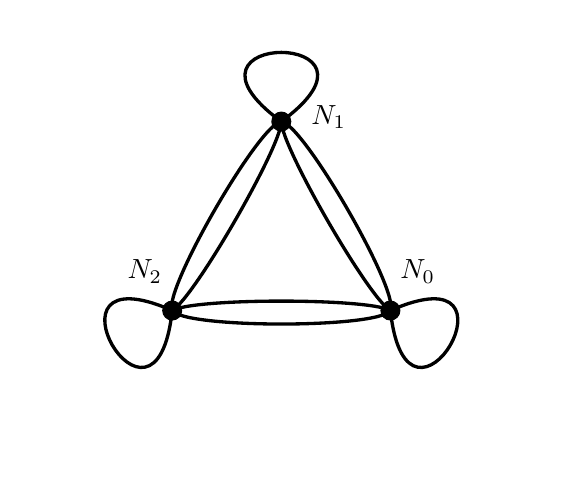
\begin{tikzpicture}[scale=0.8]
                \foreach \n in {0,...,2}{
                    \draw[very thick] ({120*\n-30}:2) .. controls ({120*\n-20}:2) and ({120*\n+120-40}:2) .. ({120*\n+120-30}:2) node[midway,sloped,allow upside down]{$\blacktriangleright$};
                    \draw[very thick] ({120*\n-30}:2) .. controls ({120*\n-30}:1.6) and ({120*\n+120-30}:1.6) .. ({120*\n+120-30}:2) node[midway,sloped,allow upside down]{$\blacktriangleleft$};
                    \draw[very thick] ({120*\n-30}:2) .. controls ({120*\n}:4) and ({120*\n-60}:4) .. ({120*\n-30}:2) node[midway,sloped,allow upside down]{$\blacktriangleright$};
                    \draw[fill=black] ({120*\n-30}:2) circle[radius=0.15];
                }
                \draw (-10:2.2) node{$N_0$};
                \draw (70:2.2) node{$N_1$};
                \draw (190:2.2) node{$N_2$};
            \end{tikzpicture}
            \caption{Quiver of the $\C\times\C^2/\Z_3$ daughter theory.}
            \label{fig:2Z3quiver}
        \end{figure}
        It is easy to see how the construction of the the quiver generalizes for arbitrary $n$. The adjacency matrix is
        \begin{equation}
            A=
            \begin{bmatrix}
                1 & \cdots & 1 \\
                \vdots & \ddots & \vdots \\
                1 & \cdots & 1
            \end{bmatrix}
        \end{equation}
        which is, as it should, coincides with the McKay decomposition of $\boldsymbol{1}\oplus\boldsymbol{2}$:
        \begin{align}
            \begin{split}
                n_{00} &= 1,\quad\dots,\qquad n_{0,n-1}=1,\\
                &\vdots\hspace{3.7cm}\vdots\\
                n_{n-1,0} &= 1,\quad\dots,\qquad n_{n-1,n-1}=1.
            \end{split}
        \end{align}
        
        Gauge anomaly cancellation now imposes that
        \begin{equation}
            N_{i-1}-N_{i-1}+N_{i+1}+N_{i+1}=0
        \end{equation}
        for $i=0,\dots,n-1$. Those constrains are always satisfied so the the factors $N_i$ are arbitrary, as long as $\sum_iN_i=N$ of course.

        This quiver is easy to scale up for any $n$. We therefore implement that into Mathematica and get the quivers for any $n$.

    \subsection{$S=\C\times\C^2/\D_n$}

        We quotient $\C^3$ by the binary dihedral group $\D_n$ that acts on the last two components. A set of irreducible representations of $\D_n$ is given by
        \begin{equation}
            \{(\rho_i,V_i)\}_{i=0,\dots,n+2}
        \end{equation}
        with $V_i=\C$ for $i=0,\dots,3$ and $V_i=\C^2$ for $i=4,\dots,n+2$, so there are $4$ one-dimensional representations and $n-1$ two-dimensional representations. They are explicitely given in section \ref{sec:irrep}. Using the bi-index notations $A_{\mu;i\alpha_i,j\beta_j}$ with $i,j=0,\dots,n+2$ and $\alpha_i,\beta_j=0,\dots,\dim\rho_i\cdot N_i-1$, the invariant configurations must have $A_{\mu;ij}=0$ if $i\neq j$, i.e. it must have a diagonal block-form, wiht block of size $\N_i\times N_i$ for $i=0,\dots,3$ and of size $2N_i\times 2N_i$ for $i=4,\dots,n+1$. The blocks transforming under the $2$-dimensional representations must have the form
        \begin{equation}
            A_{\mu;ii}=
            \begin{bmatrix}
                A_{\mu;i0,i0} & A_{\mu;i0,i1} & \cdots & A_{\mu;i,0,i,2N_i-2} & A_{\mu;i,0,i,2N_i-1} \\ 
                \mp A_{\mu;i0,i1} & A_{\mu;i0,i0} & \cdots & \mp A_{\mu;i,0,i,2N_i-1} & A_{\mu;i,0,i,2N_i-2} \\
                \vdots & \cdots & \ddots & \vdots & \vdots \\
                A_{\mu;i,2N_i-2,i,0} & A_{\mu;i,2N_i-2,i1} & \cdots & A_{\mu;i,2N_i-2,i,2N_i-2} & A_{\mu;i,2N_i-2,i,2N_i-1} \\ 
                \mp A_{\mu;i,2N_i-2,i1} & A_{\mu;i,N_i-2,i,0} & \cdots & \mp  A_{\mu;i,2N_i-2,i,2N_i-1} & A_{\mu;i,2N_i-2,i,2N_i-2}
            \end{bmatrix}
        \end{equation}
        so each block is composed of $N^2_i$ $2\times2$ matrices of the form
        \begin{equation}
            \begin{bmatrix}
                A & B \\
                \mp B & A
            \end{bmatrix}.
        \end{equation}
        We take the ``$-$'' signs when $i$ is even and the ``$+$'' signs when $i$ is odd. This comes from the fact that the $2$-dimensional representations involve alternating signs.

        R-symmetry acts on the three complex scalar fields as
        \begin{equation}
            R(A) =
            \begin{matrix}
                A
            \end{matrix}
        \end{equation}

        \marker

    \subsection{$S=\C\times\C^2/\T,\mathcal{O},\I$}

        \marker




\section{$\mN=1$ daughter theories}

    \subsection{$S=\C^3/\Z_n$}

        Let us now consider the general case of $\Z_n$ acting on $\C^3$, i.e. we want to generalize the case that we treated in section \ref{sec:C3Z3}. 
        
        \subsubsection{Actions of $\Z_n$ on $\C^3$}
        
            The first thing to do is to specify a representation of $\Z_n$ on $\C^3$. Any representation $(R,\C^3)$ can be decomposed as
            \begin{equation}
                R=\bigoplus^{n-1}_{k=0} \rho^{\oplus n_k}_k
            \end{equation}
            and is therefore equivalent to a block-diagonal representation. This implies that $\sum_kn_k=3$ so $R$ can always be written as
            \begin{equation}
                R(g)= (\rho_a\oplus\rho_b\oplus\rho_c)(g)=
                \begin{bmatrix}
                    \zeta^a_n & 0 & 0 \\
                    0 & \zeta^b_n & 0 \\
                    0 & 0 & \zeta^c_n
                \end{bmatrix}\label{eq:reprZnC3}
            \end{equation}
            with $a,b,c$ some arbitrary exponents. We denote the representation \eqref{eq:reprZnC3} by $(a,b,c)$. Let us make a few remarks on these representations:
            \begin{itemize}
                \item Since we consider $\Z_n$ as a subgroup of $\SU(3)$, we must have
                \begin{equation}
                    (a+b+c)\mod n = 0\label{eq:cdtabc}
                \end{equation}
                such that $\det(R(g))=1$.
                \item Taking $a$ or $a+n$ gives the same representation and the same is true for $b$ and $c$, so we we can actually restrict ourselves to $0<a,b,c<n$. We can trade the strict inequalities and allow the values $0$ or $n$ if we want to consider trivial representations as well. In this case, we will find that at least one direction of $\C^3$ is left untouched, i.e. we are in the situation where the orbifold is actually $\C\times\C^2/\Z_n$, which we will not consider here.
                \item Permuting $a,b,c$ gives equivalent representations so we can take $a,b,c$ to be ordered, so $0<a\leq b\leq c<n$.
            \end{itemize}

            The problem has now been reformulated as follows:
            we are looking for all possible ordered triplets $(a,b,c)$ such that $0<a\leq b\leq c<n$ and \eqref{eq:cdtabc}. For $n=1$ and $n=2$, it is clear that this is not possible, the possibilities involve at least one trivial representation. For $n=3$, the only possibility is $(1,1,1)$, the one we used in \ref{sec:C3Z3}. What about bigger values of $n$? First, note that $0<a\leq b\leq c<n$ implies that the maximum value of $a+b+c$ is $3n-1$. From equation \eqref{eq:cdtabc}, the only two possibilities are then $a+b+c=n$ or $a+b+c=2n$. What simplifies the analysis is that the second case can actually be ignored because it is already being taken care of by the first case. Let us explain that in more details: \marker
            
            Now that we have seen that the only possibility is $a+b+c=n$, we find that the maximum value that $a$ can take is $\lfloor n/3\rfloor$, so $a=1,\dots,\lfloor n/3\rfloor$. $c$ can then be expressed in terms of $a$ and $b$ as $c=n-a-b$. The constraint $b\leq c$ then implies $b\leq (n-a)/2$, i.e. $b=a,\dots,\lfloor (n-a)/2\rfloor$. To summarize, the representations are all the representations of the form
            \begin{equation}
                (a,b,n-a-b)
            \end{equation}
            with $a=1,\dots,\lfloor n/3\rfloor$ and $b=a,\dots,\lfloor (n-a)/2\rfloor$. For small values, we get
            \begin{align*}
                \Z_1 &: \text{necessarily involves a trivial representation}\\
                \Z_2 &: \text{necessarily involves a trivial representation}\\
                \Z_3 &: (1,1,1)\\
                \Z_4 &: (1,1,2)\\
                \Z_5 &: (1,1,3),(1,2,2)\label{reprZ5C3}\marker\\
                \Z_6 &: (1,1,4),(1,2,3),(2,2,2)\\
                \Z_7 &: (1,1,5),(1,2,4),(1,3,3),(2,2,3)\marker\\
                &\vdots
            \end{align*}
            For an arbitrary $n$, the total number of different representation is
            \begin{equation}
                \sum^{\lfloor n/3\rfloor}_{a=1}~\left\lfloor \frac{n-3a}{2}+1\right\rfloor = \begin{cases}
                    3k^2,\qquad\text{if $n=6k$}\\
                    3k^2+k,\qquad\text{if $n=6k+1$},\\
                    3k^2+2k,\qquad\text{if $n=6k+2$},\\
                    3k^2+3k+1,\qquad\text{if $n=6k+3$},\\
                    3k^2+4k+1,\qquad\text{if $n=6k+4$},\\
                    3k^2+5k+2,\qquad\text{if $n=6k+5$}
                \end{cases}
            \end{equation}
            The details are presented in appendix \ref{app:compsum}.

        \subsubsection{Example: $\Z_5$}

            For $\Z_5$, we saw that there are two nonequivalent ways of acting on $\C^3$, see \eqref{reprZ5C3}. Let us first consider the action $(1,1,3)$
            \begin{equation}
                R(g)=
                \begin{bmatrix}
                    \zeta_5 & 0 & 0\\
                    0 & \zeta_5 & 0\\
                    0 & 0 & \zeta^3_5
                \end{bmatrix}
            \end{equation}
            i.e. $R=\rho_1\oplus\rho_1\oplus\rho_3$.

            For the gauge field, the reasoning is exactly the same than for $\Z_3$ and we get
            \begin{equation}
                A_\mu=
                \begin{bmatrix}
                    A_{\mu;00} & & \\
                    & \ddots & \\
                    & & A_{\mu;44}
                \end{bmatrix}
            \end{equation}
            where each block $A_{\mu;ii}$ is of size $N_i\times N_i$. The projected gauge group is
            \begin{equation}
                G_{\text{proj}} = \U(N_0)\times\U(N_1)\times\U(N_2)\times\U(N_3)\times\U(N_4).
            \end{equation}

            The scalar fields transform as
            \begin{equation}
                X^m_{i\alpha_i,j\beta_j}\to R(g)\indices{^m_n}\rho_i(g)X^n_{i\alpha_i,j\beta_j}\rho_j(g)^{-1}
            \end{equation}
            so the invariant configurations must satisfy
            \begin{equation}
                X^m_{i\alpha_i,j\beta_j} = R(g)\indices{^m_n}\zeta^{i-j}_4\rho_i(g)X^n_{i\alpha_i,j\beta_j} = 
                \begin{cases}
                    \zeta^{i-j+1}X^m_{i\alpha_i,j\beta_j},\quad\text{if } m=0,1,2,3\\
                    \zeta^{i-j+3}X^m_{i\alpha_i,j\beta_j},\quad\text{if } m=4,5.
                \end{cases}
            \end{equation}
            and are therefore of the form
            \begin{equation}
                X^m = 
                \begin{bmatrix}
                    0 & X^m_{01} & 0 & 0 & 0\\
                    0 & 0 & X^m_{12} & 0 & 0\\
                    0 & 0 & 0 & X^m_{23} & 0\\
                    0 & 0 & 0 & 0 & X^m_{34}\\
                    X^m_{40} & 0 & 0 & 0 & 0
                \end{bmatrix}
            \end{equation}
            for $m=0,1,2,3$ and 
            \begin{equation}
                X^m = 
                \begin{bmatrix}
                    0 & 0 & 0 & X^m_{03} & 0\\
                    0 & 0 & 0 & 0 & X^m_{14}\\
                    X^m_{20} & 0 & 0 & 0 & 0\\
                    0 & X^m_{31} & 0 & 0 & 0\\
                    0 & 0 & X^m_{42} & 0 & 0
                \end{bmatrix}
            \end{equation}
            for $m=4,5$. Gauge anomaly cancellation imposes
            \begin{align}
                -N_{i-2}+N_{i+2}-2N_{i+1}+2N_{i-1}=0
            \end{align}
            for $i=0,1,2,3,4$ which implies that
            \begin{equation}
                N_0=N_1=N_2=N_3=N_4.
            \end{equation}

            Now if we choose the representation $(1,2,2)$, i.e.
            \begin{equation}
                R(g)=
                \begin{bmatrix}
                    \zeta_5 & 0 & 0\\
                    0 & \zeta^2_5 & 0\\
                    0 & 0 & \zeta^2_5
                \end{bmatrix}
            \end{equation}
            we get instead that the invariant field configurations must satisfy
            \begin{equation}
                X^m_{i\alpha_i,j\beta_j} = R(g)\indices{^m_n}\zeta^{i-j}_4\rho_i(g)X^n_{i\alpha_i,j\beta_j} =
                \begin{cases}
                    \zeta^{i-j+1}X^m_{i\alpha_i,j\beta_j},\quad\text{if } m=0,1\\
                    \zeta^{i-j+2}X^m_{i\alpha_i,j\beta_j},\quad\text{if } m=2,3,4,5.
                \end{cases}
            \end{equation}
            and are therefore of the form
            \begin{equation}
                X^m = 
                \begin{bmatrix}
                    0 & X^m_{01} & 0 & 0 & 0\\
                    0 & 0 & X^m_{12} & 0 & 0\\
                    0 & 0 & 0 & X^m_{23} & 0\\
                    0 & 0 & 0 & 0 & X^m_{34}\\
                    X^m_{40} & 0 & 0 & 0 & 0
                \end{bmatrix}
            \end{equation}
            for $m=0,1$ and 
            \begin{equation}
                X^m = 
                \begin{bmatrix}
                    0 & 0 &  X^m_{02} & 0 & 0\\
                    0 & 0 & 0 &  X^m_{13} & 0\\
                    0 & 0 & 0 & 0 &  X^m_{24}\\
                    X^m_{30} & 0 & 0 & 0 & 0\\
                    0 &  X^m_{41} & 0 & 0 & 0
                \end{bmatrix}
            \end{equation}
            for $m=2,3,4,5$. Gauge anomaly cancellation imposes
            \begin{align}
                -2N_{i+2}+2N_{i-2}-N_{i+1}+N_{i-1}=0\marker
            \end{align}
            for $i=0,1,2,3,4$ which implies that
            \begin{equation}
                N_0=N_1=N_2=N_3=N_4.
            \end{equation}

            \begin{figure}
                \centering
                \begin{subfigure}[b]{0.3\textwidth}
                    \centering
                    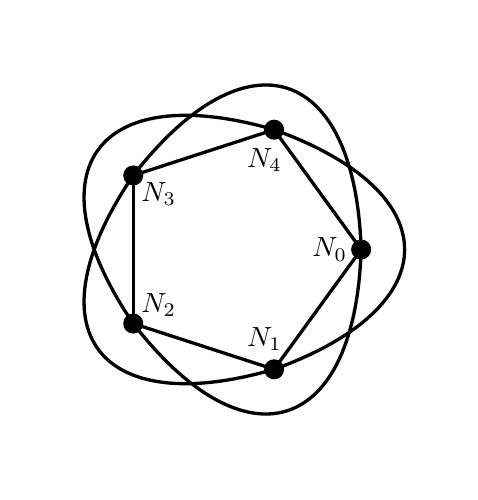
\begin{tikzpicture}[scale=0.8]
                        \foreach \n in {0,...,4}{
                            \draw[very thick] (-72*\n:2) .. controls ({-72*(\n+1)+15}:3.5) and ({-72*(\n+1)-15}:3.5) .. ({-72*(\n+2)}:2) node[midway,sloped,allow upside down]{$\blacktriangleright$};
                            \draw[very thick] ({-72*\n}:2) -- ({-72*(\n-1)}:2) node[midway,sloped,allow upside down]{$\blacktriangleright\blacktriangleright$};
                            \draw[fill=black] (-72*\n:2) circle[radius=0.15];
                            \draw (-72*\n:1.5) node{$N_\n$};
                        }
                    \end{tikzpicture}
                    \caption{$(1,1,3)$}
                    \label{fig:y equals x}
                \end{subfigure}
                \hspace{2cm}
                \begin{subfigure}[b]{0.3\textwidth}
                    \centering
                    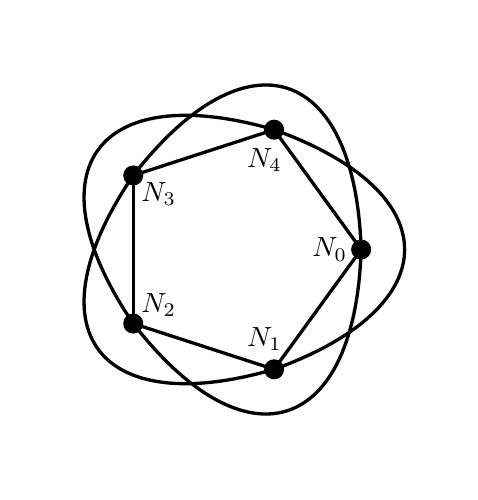
\begin{tikzpicture}[scale=0.8]
                        \foreach \n in {0,...,4}{
                            \draw[very thick] (-72*\n:2) .. controls ({-72*(\n+1)+15}:3.5) and ({-72*(\n+1)-15}:3.5) .. ({-72*(\n+2)}:2) node[midway,sloped,allow upside down]{$\blacktriangleleft\blacktriangleleft$};
                            \draw[very thick] ({-72*\n}:2) -- ({-72*(\n-1)}:2) node[midway,sloped,allow upside down]{$\blacktriangleright$};
                            \draw[fill=black] (-72*\n:2) circle[radius=0.15];
                            \draw (-72*\n:1.5) node{$N_\n$};
                        }
                    \end{tikzpicture}
                    \caption{$(1,2,2)$}
                    \label{fig:three sin x}
                \end{subfigure}
                \caption{Quivers of the $\C^3/\Z_5$ daughter theories.}
                \label{fig:Z5graphs}
           \end{figure}

           Note that, even we thought that $(1,1,3)$ and $(1,2,2)$ were different representation, that are actually equivalent in the sense that $(1,1,3)+(1,1,3)=(2,2,1)$. The two quivers in fig. \ref{fig:Z5graphs} should therefore be the same. And indeed, upon further inspection, the two are the same. To see this, we can rename the vertices in the second graph as $N_1\to N_3,N_2\to N_1,N_3\to N_4,N_4\to N_2$. This renaming defines the bijection between the two graphs. A more pragmatic way to see this is to look at the adjacency matrices:
           \begin{equation}
                a_{(1,1,3)}=
                \begin{bmatrix}
                    0 & 0 & 1 & 0 & 2 \\
                    2 & 0 & 0 & 1 & 0 \\
                    0 & 2 & 0 & 0 & 1 \\
                    1 & 0 & 2 & 0 & 0 \\
                    0 & 1 & 0 & 2 & 0
                \end{bmatrix}\qquad
                a_{(1,2,2)}=
                \begin{bmatrix}
                    0 & 0 & 0 & 2 & 1 \\
                    1 & 0 & 0 & 0 & 2 \\
                    1 & 1 & 0 & 0 & 0 \\
                    0 & 2 & 1 & 0 & 0 \\
                    0 & 0 & 2 & 1 & 0
                \end{bmatrix}.
           \end{equation}
           Changing the names of the vertices is equivalent to swapping line and columns. For example, 

        \subsubsection{General $\Z_n$}

           Let us now consider the general action
           \begin{equation}
                R(g)=
                \begin{bmatrix}
                    \zeta^a_n & 0 & 0\\
                    0 & \zeta^b_n & 0\\
                    0 & 0 & \zeta^c_n
                \end{bmatrix}
           \end{equation}
           of $\Z_n$ on $\C^3$, where $(a,b,c)$ one of the representation that we studied before. In particular, recall that $a+b+c=n$. Following the same reasoning than before, we get that the gauge field of of the form
           \begin{equation}
               A_\mu=
               \begin{bmatrix}
                   A_{\mu;00} & & \\
                   & \ddots & & \\
                   & & A_{\mu;n-1,n-1}
               \end{bmatrix}.
           \end{equation}

           Invariant scalar field configurations transform as
           \begin{equation}
               X^m_{i\alpha_i,j\beta_j}=
               \begin{cases}
                   \zeta^{i-j+a}_nX^m_{i\alpha_i,j\beta_j},\qquad \text{if }m=0,1\\
                   \zeta^{i-j+b}_nX^m_{i\alpha_i,j\beta_j},\qquad \text{if }m=2,3\\
                   \zeta^{i-j+c}_nX^m_{i\alpha_i,j\beta_j},\qquad \text{if }m=4,5
               \end{cases}
           \end{equation}
           so
           \begin{align}
               X^{0,1}_{j-a,j} &\in (\boldsymbol{\textbf{N}_j},\boldsymbol{\bar{\textbf{N}}_{j-a}}),\\
               X^{2,3}_{j-b,j} &\in (\boldsymbol{\textbf{N}_j},\boldsymbol{\bar{\textbf{N}}_{j-b}}),\\
               X^{4,5}_{j-c,j} &\in (\boldsymbol{\textbf{N}_j},\boldsymbol{\bar{\textbf{N}}_{j-c}})
           \end{align}
           are the only possible non-vanishing components. This allows us to quickly draw all the possible quivers for a given $n$. Once again, the difficulty is only computational, not conceptual. This can therefore easily be implemented into Mathematica and we get the quiver for any $n$ and any representation $(a,b,c)$.
        
    \subsection{$S=\C^3/\Delta(3n^2),\Delta(6n^2)$}

    \subsection{$S=\C^3/\Sigma_{36\times 3},\Sigma_{60\times 3},\Sigma_{168\times 3},\Sigma_{216\times 3},\Sigma_{360\times 3}$}

    \subsection{$S=\C^3/(\Z_m\times\Z_n)$}

        \subsubsection{Representations of $\Z_m\times\Z_n$}

           We consider the group $\Z_m\times\Z_n$. Let us denote by $\{\mu_i\}_{i=0,\dots,m-1}$ and $\{\sigma_j\}_{j=0,\dots,n-1}$ two complete set of irreducible representation of $\Z_m$ and $\Z_n$ respectively, with
           \begin{align}
               \mu(g_1)&=\zeta^i_m\\
               \sigma_j(g_2)&=\zeta^j_n
           \end{align}
           where $g_1$ and $g_2$ are the generating elements of $\Z_m$ and $\Z_n$ respectively. $\Z_m\times\Z_n$ is of order $mn$ and possesses the same number of equivalency classes (abelian). It has therefore $mn$ irreducible representations. Since the group is abelian, they are all of dimension $1$. Let us denote by $\{T_k\}_{k=0,\dots,m+n-1}$ a complete set of irreducible representations. Since we have a product group, for any $k$ there exists indices $i(k)$ and $j(k)$ such that $T_k=\mu_{i(k)}\otimes\sigma_{j(k)}$. We choose the indices $i(k)$ and $j(k)$ such that
           \begin{align*}
               T_0 &= \mu_0\otimes\mu_0,\\
               T_1 &= \mu_0\otimes\mu_1,\\
               T_2 &= \mu_0\otimes\mu_2,\\
               &\vdots\\
               T_{n-1} &= \mu_0\otimes\mu_{n-1},\\
               T_n &= \mu_1\otimes\mu_0,\\
               &\vdots\\
               T_{2n-1} &= \mu_1\otimes\mu_{n-1},\\
               &\vdots\\
               T_{mn-1} &= \mu_{m-1}\otimes\mu_{n-1}.
           \end{align*}
           That is, we take
           \begin{equation}
               \begin{cases}
                   i(k) &= \lfloor k/n\rfloor\\
                   j(k) &= k\mod n
               \end{cases}\qquad \Leftrightarrow \qquad k=i(k)n+j(k).
           \end{equation}
           Note that this simply a dictionary between a line notation and a matrix notation and that it is indeed a bijection $k\Leftrightarrow i,j$. In this way, we can proceed to similar manipulations than before, were we used line notations. 

           Any representation $R$ of $\Z_m\times\Z_n$ can be decomposed as
           \begin{equation}
               R=\bigoplus_{i,j}N_k T_k=\bigoplus_{i,j}N_{ij}(\mu_{i}\otimes\sigma_{j})
           \end{equation}
           with $N_k=N_{i(k)j(k)}$. We must have $\sum_kN_k=3$. In other words, any representation of $\Z_m\times\Z_n$ on $\C^3$ is equivalent to
           \begin{equation}
                R(g_1,g_2)=[(\mu_{a}\otimes\sigma_{a'})\oplus(\mu_{b'}\otimes\sigma_{b'})\oplus(\mu_{c}\otimes\sigma_{c'})](g_1,g_2)=
               \begin{bmatrix}
                   \xi^a_m\xi^{a'}_n & 0 & 0 \\
                   0 & \xi^b_m\xi^{b'}_n & 0 \\
                   0 & 0 & \xi^c_m\xi^{c'}_n
               \end{bmatrix}.
           \end{equation}
           The determinant condition is
           \begin{align}
                \xi^{a+b+c}_m &= \xi^{-a'-b'-c'}_n\\
               \Leftrightarrow (a+b+c)\mod m &= (a'+b'+c')\mod n
           \end{align}

           

           \begin{equation}
            R(g_1,g_2)=
           \begin{bmatrix}
               \xi_m & 0 & 0 \\
               0 & \xi_n & 0 \\
               0 & 0 & \xi^{-1}_m\xi^{-1}_n
           \end{bmatrix}.
       \end{equation}

    \subsubsection{Projection}

        Let us start by the gauge field. We consider a unitary representation $(\rho,\C^N)$ of $\Z_m\times \Z_n$ on $\C^n$ and decompose it as
        \begin{equation}
            \rho=\bigoplus_{i,j}N_k T_k
        \end{equation}
        such that
        \begin{equation}
            \rho(g)=
            \begin{bmatrix}
                T_0(g) & & & \cdots & & & 0 \\
                & \ddots & & & & & \\
                & & T_0(g) & & & &  \\
                \vdots & & & \ddots & & & \vdots \\
                & & & & T_{mn-1}(g) & & \\
                & & & & & \ddots & \\
                0 & & & \cdots & & & T_{mn-1}(g) 
            \end{bmatrix}
            \hspace{-0.2cm}
            \begin{tabular}{l}
            $\left.\lefteqn{\phantom{
                \begin{matrix}
                    a_0\\ \ddots\\ a_0\ 
                \end{matrix} 
            }}\right\}N_0$\\
            \vdots \\
            $\left.\lefteqn{\phantom{
                \begin{matrix}
                    b_0\\ \ddots\\ b_0\ 
                \end{matrix}
            }} \right\}N_{mn-1}$
            \end{tabular}.
        \end{equation}

        We can now use our usual bi-index notation $A_{\mu;k\alpha_k,l\beta_l}$ with $k,l=0,\dots mn-1$ and $\alpha_k,\beta_k=0,\dots,N_k$ but instead it is more convenient to come back to our matrix notation by writing the block $A_{\mu;k,l}$ as $A_{\mu;i(k)j(k),i(l)j(l)}$ that we simply denote by $A_{\mu;ij,i'j'}$ with $i,i'\in\{0,\dots,n-1\}$ and $j,j'\in\{0,\dots,n-1\}$. So for $m=2,n=3$ for example, the link between the two notations is
        {\tiny
        \begin{equation}
            \begin{bmatrix}
                A_{\mu;00} & A_{\mu;01} & A_{\mu;02} & A_{\mu;03} & A_{\mu;04} & A_{\mu;05} \\
                A_{\mu;10} & A_{\mu;11} & A_{\mu;12} & A_{\mu;13} & A_{\mu;14} & A_{\mu;05} \\
                A_{\mu;20} & A_{\mu;21} & A_{\mu;22} & A_{\mu;23} & A_{\mu;24} & A_{\mu;05} \\
                A_{\mu;30} & A_{\mu;31} & A_{\mu;32} & A_{\mu;33} & A_{\mu;34} & A_{\mu;05} \\
                A_{\mu;40} & A_{\mu;41} & A_{\mu;42} & A_{\mu;43} & A_{\mu;44} & A_{\mu;05} \\
                A_{\mu;50} & A_{\mu;51} & A_{\mu;52} & A_{\mu;53} & A_{\mu;54} & A_{\mu;05}
            \end{bmatrix}=
            \begin{bmatrix}
                \begin{bmatrix}
                    A_{\mu;00,00} & A_{\mu;00,01} & A_{\mu;00,02}\\
                    A_{\mu;01,00} & A_{\mu;01,01} & A_{\mu;01,02}\\
                    A_{\mu;02,00} & A_{\mu;02,01} & A_{\mu;02,02}\\
                \end{bmatrix}
                \begin{bmatrix}
                    A_{\mu;00,10} & A_{\mu;00,11} & A_{\mu;00,12}\\
                    A_{\mu;01,10} & A_{\mu;01,11} & A_{\mu;01,12}\\
                    A_{\mu;02,10} & A_{\mu;02,11} & A_{\mu;02,12}\\
                \end{bmatrix}\\
                \begin{bmatrix}
                    A_{\mu;10,00} & A_{\mu;10,01} & A_{\mu;10,02}\\
                    A_{\mu;11,00} & A_{\mu;11,01} & A_{\mu;11,02}\\
                    A_{\mu;12,00} & A_{\mu;12,01} & A_{\mu;12,02}\\
                \end{bmatrix}
                \begin{bmatrix}
                A_{\mu;10,10} & A_{\mu;10,11} & A_{\mu;10,12}\\
                A_{\mu;11,10} & A_{\mu;11,11} & A_{\mu;11,12}\\
                A_{\mu;12,10} & A_{\mu;12,11} & A_{\mu;12,12}\\
            \end{bmatrix}
            \end{bmatrix}
        \end{equation}}
        So instead of considering $A_\mu$ to be a single $mn\times mn$ matrix of element $A_{\mu;kl}$, where $A_{\mu;kl}$ are $N_k\times N_l$ matrices, we consider it as an $m\times m$ where each element $A_{\mu,ii'}$ (line $i$ column $i'$) is itself an $n\times n$ matrices with elements $A_{\mu;ij,i'j'}$ (line $j$ column $j'$), as shown above.

        Using these notations, the gauge field transforms as
        \begin{equation}
            A_{\mu;ij,i'j'} \mapsto (\mu_i(g)\otimes\sigma_j(g))A_{\mu;ij,i'j'}(\mu_{i'}(g)\otimes\sigma_{j'}(g))^{-1} = \zeta^{i-i'}_m\zeta^{j'-j}_n A_{\mu;ij,i'j'}
        \end{equation}
        so invariant configurations can possess non-vanishing components $A_{\mu;ij,i'j'}$ only if
        \begin{align}
            \zeta^{i-i'}_m &= \zeta(j'-j)_n \\
            \Leftrightarrow\quad (i-i')\mod m &= (j'-j)\mod n \\
            \Leftrightarrow\quad j' &= j+\abs{i'-i}.
        \end{align}
        This means that the submatrices $A_{\mu;ii'}$ has an off-diagonal block form with offset $\abs{i'-i}$. Once again, for a general $n$, the difficulty is only computational, not conceptual. This can therefore easily be implemented into Mathematica and we get the form of the gauge field for any $n$.

        For the scalar fields, we have
        \begin{align}
            X^m_{ij,i'j'}&\mapsto R(g)\indices{^m_n}(\mu_i(g)\otimes\sigma_j(g))X^n_{ij,i'j'}(\mu_{i'}(g)\otimes\sigma_{j'}(g))^{-1}\\
            &\quad =
            \begin{cases}
                \zeta^{i-i'+1}_m\zeta^{j-j'}_n X^m_{ij,i'j'},\qquad m=0,1\\
                \zeta^{i-i'}_m\zeta^{j-j'+1}_n X^m_{ij,i'j'},\qquad m=2,3\\
                \zeta^{i-i'-1}_m\zeta^{j-j'-1}_n X^m_{ij,i'j'},\qquad m=4,5.
            \end{cases}
        \end{align}
        So a configuration is invariant if and only if the only non-vanishing component satisfy
        \begin{align}
            m=0,1 &: (i-i'+1)\mod m = (j'-j)\mod n\\
            m=2,3 &: (i-i')\mod m = (j'-j-1)\mod n\\
            m=4,5 &: (i-i'-1)\mod m = (j'-j+1)\mod n.
        \end{align}

\section{Correspondence between gauge theory and singularity}

    Above, we presented all the possible orbifold constructions of supersymmetric quiver gauge theories in four dimensions. We started from quotienting the transverse space and we found the corresponding (supersymmetric) gauge theory. In other words, we started from the singularity a found the gauge theory. We can therefore consider that the orbifold singularities are understood. However, not all singularities are orbifold one, such as the conifold for example. We can then ask ourselves how to obtain the gauge theory for more general singularities than the orbifold ones. Is a general approach possible ? On the other hand, we can also study the converse question; is it possible to to obtain the singularity from the gauge theory? And if it is, how so? In general we will see that there is a bijection between the four-dimensional supersymmetric worldvolume gauge theory and the Calabi-Yau singularity. We now detail this bijection.

    \subsection{From gauge theory to singularity: forward algorithm}

        We start with the simplest question: how to recover the singularity from the gauge theory? We already mentioned that the vacuum parameter space of the scalar fields of the gauge theory is the so-called moduli space, denoted $\M$. Because our D$3$-brane is a point in the Calabi-Yau threefold, the vacuum moduli space $\M$ is the affine coordinates of the Calabi-Yau singularity $S$.

        For the ADE $\mN=2$ theories discussed in section \ref{sec:N2QGT}, by the Kronheimer-Nakajima construction \cite{Kronheimer1990}, the moduli space is a hyper-Kähler quotient. In general, the moduli space can be constructed as a \emph{quiver variety}, i.e. a variety constructed from the moduli space of quiver a quiver representation. More rpecisely, given the dimensions of the vector spaces assigned to every vertex, one can form a variety which characterizes all representations of that quiver with those specified dimensions, and consider stability conditions. Let us see some examples of this.

        The anomaly free condition is
        \begin{equation}
            (a_{ij}-a_{ji})n_i=0\marker.
        \end{equation}

        \subsubsection{$S=\C\times\C^2/\Z_n$}

        \subsubsection{The conifold}

    \subsection{From singularity to gauge theory: inverse algorithm}

        Mathematically, a quiver gauge theory is a representation of a finite quiver with relations. The labels are $\{N_i\in\Z_+\}$, they correspond to the dimension of the vector space $\{V_i\}$. The gauge group is $\prod_i\SU(N_i)$. The gauge fields are self-adjoint arrows $\Hom(V_i,V_i)$ while the matter fields are bi-fundamentals fermions/bosons and are arrows $X_{ij}\in\Hom(V_j,V_i)$. For a quiver with adjacency matrix $a_{ij}$, the gauge anomaly cancellation condition can be generally expressed as
        \begin{equation}
            (a_{ij}-a_{ji})N_i=0.
        \end{equation}
        At last, there are some relations that arises the superpotential $W(\{X_{ij}\})$. The vacuum is the minima of the superpotential. In other words,
        \begin{equation}
            \pdv{W}{X_{ij}}=0.
        \end{equation}

\section{A note about projective representations, discrete torsion and deformations}

    \subsection{Projective representations and discrete torsion}

        Up until now, and in particular in all of our computations in section \ref{sec:orbsing}, we only considered ordinary representations, i.e. linear representations. We can however use a more general representations such as projective representations for example. That is, representations $\rho$ of $\Gamma$ such that for all $\gamma_1,\gamma_2\in\Gamma$,
        \begin{equation}
            \rho(\gamma_1)\rho(\gamma_2)=A(g_1,g_2)\rho(\gamma_1\gamma_2)
        \end{equation}
        for some factor $A(\gamma_1,\gamma_2)$. The $A(\gamma_1,\gamma_2)=1$ corresponding to linear representations. For consistency reasons, the factor $A(g_1,g_2)$ cannot be completely arbitrary and must a cocycle condition. As a result, the possibilities for $A(\gamma_1,\gamma_2)$ are classified by the second cohomology group $H^2(\Gamma,\C^*)$, also called \emph{discrete torsion}. There exists a projective representation if and only if the latter does not vanish. This new liberty, whenever admissible, provides new classes of quiver gauge theories that can be remarkably different from the ones we considered up until now, with no discrete torsion.

        What happens is that if one turns on an NSNS B-fiels alors the worldvolume, then the moduli space is expected to a non-commutative version of a Calabi-Yau space. This haw the discrete torsion is physically realized. Another, and actually equivalent through T-duality, way of studying gauge theories is to consider D-branes streched between configurations of NS$5$-branes\footnote{D$5$-branes are charged under the Ramond-Ramond field whose quanta comes from the Ramond-Ramond sector but NS$5$-branes are charges under the Kalb-Ramonf field whose quanta comes fromthe Neveu-Schwarz. On the worldvolume of an NS$5$-brane (6-dimensional) propagates propagates a superstring, this called the \emph{little string}.}. This is the\emph{Hanany-Witten setup}.

        The discrete tosrion also appears when writing the full open strin gpartition function that inclues the \emph{twisted sector}\footnote{The twisted sector is subspace of the full Hilbert space of string states in a particular theory over a (good) orbifold.} where there is ambiguity up to a phase factor. As a consequence from modular invariance, the latter must satisfy certain cocycle conditions. It is precisely the deiscrete torsion. Note that this has been found to be true only for the open string sector.

    \subsection{Quiver gauge theories deformations and conifold}

        We can deforming the singular algebraic description of the orbifold with a field into a family smooth surfaces. The resulting total space is the \emph{conifold}.

\part{Beyond orbifold singularities}

\section{Non-commutative resolutions}

\section{Determinantal varieties as transverse spaces}

    \subsection{Basic properties of determinantal varieties}  

            A \emph{determinantal variety} (DV) is a space of matrices with a given upper bound on their ranks. More precisely, given $m,n$ and $r<\min(m,n)$, the DV $Y_r$ of the field $K$ is the set of $m\times n$ matrices over $K$ with rank lower or equal to $r$:
            \begin{equation}
                Y_r\equiv\{M\in M_{m\times n}(K)|\rank M\leq r\}.
            \end{equation}
            Recall that a $k$-minor is the determinant of a $k\times k$ sub-matrix and that the rank of a matrix is equal to the biggest integer such that there is a non-vanishing minor of that size. Imposing $\rank M\leq r$ is therefore equivalent to the vanishing of its $(r+1)\times (r+1)$ minors, as it also implies tha vanishing of the biggest minors. This naturally qualifies $R_r$ as affine varieties embedded in $K^{mn}$. Let us denote by $x_{i,j}$ the independent entries of a generic matrix of $Y_r$, i.e. $x_{i,j}$ are affine coordinates. The minors are therefore homogeneous polynomials of degree $r+1$. The ideal of $K[x_{i,j}]$ generated by these polynomials $(r+1)\times(r+1)$ is called the \emph{determinantal ideal}. Homogeneity the polynomials implies that $Y_r$ can equivalently be seen as a projective variety in $\bbA^{mn-1}$.

        \subsubsection{Computing the dimension}
            
            Let us compute the dimension of $Y_r$ seen as an affine variety. We consider the space $\bbA^{mn}\times\textbf{Gr}(r,m)$, where $\textbf{Gr}(r,m)$ is the Grassmannian of $r$-planes in an $m$-dimensioanl vector space. Let us define the subsapce
            \begin{equation}
                Z_r\equiv\{(A,W)|Ax\in W\text{ for all } x\in\bbA^{n}\}.
            \end{equation}
            $Y_r$ and $Z_r$ are birationaly equivalent so $\dim Y_r=\dim Z_r$. We want to compute $Z_r$. First we notice that $Z_r$ is a vector bundle over $\textbf{Gr}(r,m)$ and we denote it by $Z_r\xrightarrow[]{\pi_1}\textbf{Gr}(r,m)$. Now, over the Grassmannian $\textbf{Gr}(r,m)$, there is a tautologial vector bundle that we denote by $E_{\textbf{Gr}}\xrightarrow[]{\pi_2}\textbf{Gr}(r,m)$ whose fibers are $\pi^{-1}_2(W)=W\cong\R^r$. Finally, $K^m$ can also be seen as a vector bundle, with fibers $\R^m$. We denote it by $E_{K^n}\xrightarrow[]{\pi_3}K^n$. From $E_{\textbf{Gr}}$ and $E_{K^n}$, we can construct\footnote{Recall that if $E$ and $F$ are vector bundles over $X$, then we can construct a new vetor bundle over $X$, called the Hom-bundle and denoted $\Hom(E,F)$, by defining the fiber over $x\in X$ to be $\Hom(E_x,F_x)$.} the vector bundle $\Hom(E_{\textbf{Gr}},E_{K^n})\xrightarrow[]{\pi_4}\textbf{Gr}(r,m)$. This vector bundle has the same base space and its fibers are $\Hom(\R^m,\R^r)$ which are exactly the same as the ones of $Z_r$. So the two vector bundles are isomorphic:
            \begin{equation}
                Z_r\cong\Hom(E_{\textbf{Gr}},E_{K^n}).
            \end{equation}
            Finally, since the fibers of $\Hom(K^n,E_{\textbf{Gr}})$ have dimension $nr$, we find
            \begin{equation}
                \dim Z_r = \dim\Hom(K^n,E_{\textbf{Gr}}) = \dim\textbf{Gr}(r,m)+nr = r(m-r)+nr.
            \end{equation}
            Finally, we conclude that $Y_r$ is a affine variety of dimension $r(m-r)+nr$.

            \begin{table}[H]
                \centering
                $
                \begin{array}{|c|c|c||c|}
                    \hline
                    m & n & r & \dim_\C Y_r \\ \hline
                    2 & 2 & 1 & 3 \\ \hline
                    3 & 2 & 1 & 4 \\ \hline
                    3 & 3 & 1 & 5 \\ \hline
                    3 & 3 & 2 & 8 \\ \hline
                    4 & 2 & 1 & 5 \\ \hline
                    4 & 3 & 1 & 6 \\ \hline
                    4 & 3 & 2 & 10 \\ \hline
                    4 & 4 & 1 & 7 \\ \hline
                    4 & 4 & 2 & 12 \\ \hline
                    4 & 4 & 3 & 15 \\ \hline
                \end{array}
                $
            \end{table}

        \subsubsection{Singularity}
        
            The varitey $Y_r$ is singlar and the singular locus is contained in the subset of matrices with rank strictly lower than $r$. $Z_r$ is a resolution (over the open set of matrices with rank exactly $r$, this map is an isomorphism)\marker.

        \subsubsection{Action and syzygies}

            $Y_r$ naturally acts on $G=\GL(m,K)\times\GL(n,K)$

        \subsection{Young's lattice}

            \emph{Young's lattice} is a lattice $Y$ formed by all integer partitions ordered by inclusion of their Young tableau. It is generally used to 

            \begin{figure}[H]
                \centering
                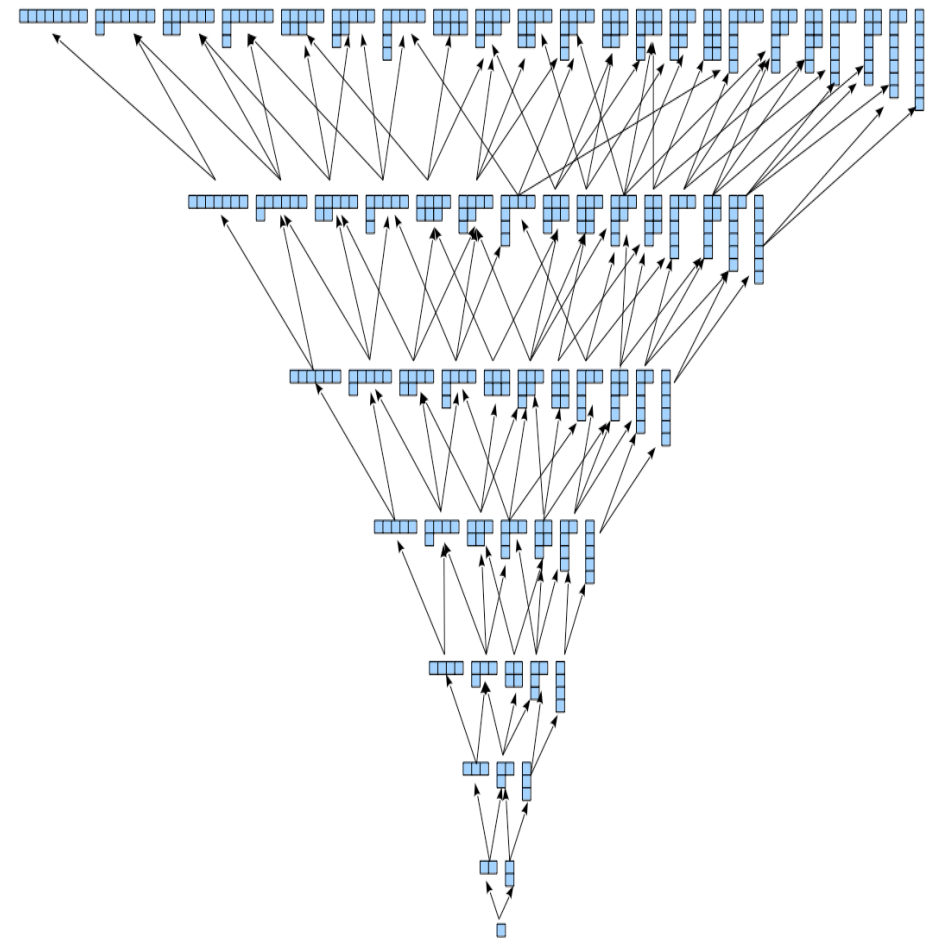
\includegraphics[scale=0.35]{Pictures/youngslattice.png}
                \caption{Young's lattice depicted as a Hasse diagram, i.e. the descendance of two tableaux is the union and the parent is the intersection.}
            \end{figure}


        



\pagebreak
\appendix

\section{Simplicial Homology}

    An \emph{$n$-simplex}, denoted by $\Delta^n=[v_0,\dots,v_n]$ is the smallest convex set in $\R^m$ containing $n+1$ points $v_0,\dots,v_n$ that do not lie in a hyperplane of dimension less than $n$. Or, equivalently, such that $v_1-v_0,\dots,v_n-v_0$ are linearly independant. The $n+1$ point $v_0,\dots,v_n$ are the \emph{vertices} of the $n$-simplex. A by-product of our ordered notation for the vertices of a simplex is that it determines an orientation for the edges $[v_i,v_j]$ according to the increasing subscripts. The \emph{faces} of an $n$-simplex are all the sub-simplices that can obtained by removing vertices of the original simplex. The order of the vertices of the smaller simplices is taken to be same than in the original $n$-simplex. 
    
    Let us now put some simplices together. If $X$ be a topological space, then a \emph{simplicial complex structure} $\Delta$ on $X$ is a collection $\Delta=\{\sigma_\alpha\}$ of continuous maps $\sigma_\alpha:\Delta^{n(\alpha)}\to X$ called \emph{characteristic maps} such that
    \begin{enumerate}[label=\roman*)]
        \item $\sigma_\alpha|_{e^{n(\alpha)}}$ is injective and that for all $x\in X$ there exists $\alpha$ such that $x\in\Im(\sigma_\alpha|_{e^{n(\alpha)}})$,
        \item the restriction of any map $\sigma_\alpha$ to a face of $\Delta^n$ is another $\sigma_\beta$,
        \item for any subset $A\subseteq X$, $A$ is open if and only if $\sigma^{-1}_{\alpha}(A)$ is open in $\Delta^n$ for all $\alpha$,
    \end{enumerate}
    where $\Delta^n$ is an $n$-simplex and $e^n$ is the interior of $\Delta^n$. 

    Given a simplicial complex structure $\Delta$ on $X$, $n$-chains are finite formal sums
    \begin{equation}
        \sum_\alpha n_\alpha \sigma_\alpha(e^{n(\alpha)})
    \end{equation}
    with coefficient $n_\alpha\in\Z$. We denote by $\Delta_n(X)$ the set of all $n$-chains, it is a free abelian group.

    For a general simplicial complex structure on $X$, we define a \emph{boundary homomorphism} $\p_n:\Delta_n(X)\to\Delta_{n-1}(X)$ by its action on the basis elements:
    \begin{equation}
        \p_n(\sigma_\alpha)=\sum_i(-1)^i\sigma_\alpha|_{[v_0,\dots,\hat{v_i},\dots,v_n]}.
    \end{equation}
    In particular, homomorphism here means that this maps are linear. We can note that the right side of this equation does indeed lies in $\Delta_{n-1}(X)$ since each restriction $\sigma_\alpha|_{[v_0,\dots,\hat{v_i},\dots,v_n]}$ is the characteristic map of an $(n-1)$-simplex of $X$. The most important property of those maps is that $\p_{n}\circ\p_{n+1}=0$ (symbolically $\p^2=0$), meaning that $\Im\p_{n+1}\subset\Ker\p_n$. We can then form a sequence of homomorphisms of abelian groups
    \begin{equation}
        \dots\to \Delta_{n+1}(X)\xrightarrow[]{\p_{n+1}}\Delta_n(X)\xrightarrow[]{\p_{n}}\Delta_{n-1}(X)\to\dots\to\Delta_1(X)\xrightarrow[]{\p_{1}}\Delta_0(X)\to 0
    \end{equation}
    $\Im\p_{n+1}\subset\Ker\p_n$ for each $n$. Chains of homomorphisms satisfying this property are called \emph{chain complex}. We have extended the chain at the end with $\p_0=0$ such that this property is also true at the ends. Elements of $\Ker\p_n$ are called \emph{$n$-cycles} and elements of $\Im\p_{n+1}$ are called \emph{$n$-boundaries}. Note that they are each elements of $\Delta_n(X)$, hence the notation. 
    \begin{examp*}
        If we consider a triangle withe vertices $A,B$ and $C$, we can put a simplicial complex structure on it consisting of one $2$-simplex ($u=[A,B,C]$), three 1-simplices ($a=[A,B],b=[B,C],c=[C,A]$) and three $0$-simplices ($A,B,C$). We can see that
        \begin{equation}
            \p_2(u)=[B,C]-[A,C]+[A,B] = a+b+c.
        \end{equation} 
        So we get that $a+b+c$ is a $1$-boundary. However, we see that
        \begin{equation}
            \p_1(a+b+c)=B-A+C-B+A-C=0
        \end{equation}
        so it is also a $1$-cycle.
    \end{examp*}
    The fact that image of each map lies the kernel of the next map means that any boundary is also a cycle. As illustrated by the previous example. We can wonder what are the cycles that are not boundaries of any higher-dimensional simplicial complex. This set is precisely the quotient space
    \begin{equation}
        H_n(X)=\frac{\Ker(\p_n)}{\Im\p_{n+1}}.
    \end{equation}
    It naturally inherits a group structure and is called the $n$th \emph{Homology group} of $X$. The elements of this space are equivalence classes (cosets of $\Im\p_{n+1}$) of $n$-cycles where two cycles are considered equivalent if they only differ by a boundary, i.e. if their formal difference is a boundary. These equivalence classes are called \emph{homology classes}.

    \begin{examp*}
        Let us give some useful examples of Homology groups for various topological spaces:
        \begin{itemize}
            \item the Homology groups of $\R^n$ are all trivial therefore $\chi=0$.
            \item the non-trivial Homology groups of the $n$-sphere are $H_0(S^n)=H_n(S^n)=\Z$ therefore $\chi=(-1)^n-1$
            \item the only non-trivial Homology group of the $n$-ball is $H_0(B^n)=\Z$ therefore $\chi=1$.
            \item the non-trivial Homology groups of the $2$-torus are $H_0(T)=H_2(T)=\Z$ and $H_1(T)=\Z^2$ therefore $\chi=(1+x)^2$.
            \item the non-trivial Homology groups of the complex projective space are $H_{0\leq 2k\leq 2n}(\C\P^n)=\Z$.
            \item the only non-trivial Homology groups of any Riemann surface of genus $g$ are $H_0=\Z, H_1=\Z^{2g}$ and $H_2=\Z$, such that $\chi=2-2g$.
        \end{itemize}
    \end{examp*}
    Let us make a comment on the zeroth homology group. Since $\Ker\p_0=\Delta_0$ by definition, all elements of $\Delta_0$ (i.e. every point of $X$) are $0$-cycles and $H_0(X)$ is the set of $0$-cycles that are not the boundary of any chain of $1$-simplices. Since any linear combination of $0$-simplices (i.e. point) can be seen as the boundary the $1$-simples that joins them, we can see that all points that can be joined by a path are equivalent. For a topological space $X$ where all points can be connected by a path this means that the zeroth homology group is necessarily $H_{0}(X)=\{nA|a\in\Z\}\cong\Z$, where $A$ any point in $X$. More generally, we can conclude that the number of copies of $\Z_n$ in $H_0(X)$ is the number of path-connected components of $X$.

    For a graph $\Gamma$, we can understand from our previous discussions that the only non-trivial homology groups are going to be $H_0(\Gamma)=\Z\times\dots\times\Z$ where the number of copies is the number of connected components and $H_1(\Gamma)=\Z\times\dots\times\Z$ where the number of copies is the number of ``irreducible'' loops.

    The $n$th simplicial homology group of a topological space $X$ with a complex simplicial structure $\Delta$ is always of the form
    \begin{equation}
        H^\Delta_n(X)=\underbrace{\Z\times\Z}_{b_n}\oplus\Z_{q_1}\times\dots\times\Z_{q_s}.
    \end{equation}
    $b_n$ are the Betti numbers. The \emph{Poincaré polynomial} is
    \begin{equation}
        P_X(x)=\sum_{i\geq 0}b_ix^i
    \end{equation}
    and the Euler characteristic of $X$ is given by $P_X(-1)$. Recall that the Euler characteristic is also given by $\chi=2-2g-b-c$, $g$ being the genus, $b$ the number of topological boundaries and $c$ the number of crosscaps.

    Note that the homology that we considered is with coefficients in $\Z$, i.e. we started with simplicial chains with coefficients in $\Z$. We can however also consider coefficients in $\R$, in $\C$ or in any ring. In those case however we can easily lose the information about torsion. For example $\Z/2\Z=\Z_2$ is non trivial but since $2\R=\R$, $\R/2\R=\{0\}$.

\section{Spacetime geometry: ALE space and orbifolds}\label{app:spacetimegeom}

    Asymptotically locally euclidean (ALE) spaces are a particularly interresting choice of string background to probe with branes for mainly four reasons
    \begin{enumerate}[label=(\roman*)]
        \item they are the resolution (blow-ups) of orbifolds
        \item there are completely classified: they fall in the ADE classification
        \item they only break half of the supersymmetry
        \item they are non-compact therefore we can study them for self-dual type II theory. \todo{Why is that ?}
    \end{enumerate}
    Mathematically, an ALE space is complete riemannian $n$-manifold $M$ such that there exists a compact set $K\subset M$ such that $M\backslash K$ is diffeomorphic to $(\R^n\backslash B_0(R))/G$, where $R\in\R^+_0$ is a radius and $G\subset\O(n)$ a subgroup. Additionally, it is asked that the pulled back metric on $\R^n\backslash B_0(R)$ tends to the euclidean flat metric at infinity.

    If one considers string theory an the orbifold $\R^4/\Gamma$ where $\Gamma$ is a finite sub group of $\SU(2)$, massless states appear from the twisted sector. They are precisely the moduli needed the deform the theory to the one with smooth spacetime, i.e. the resolution of the orbifold. In that sense, is said that the strings know about the metric ALE space and that it is said that strings resolve the singularity. The metric of the ALE space can be recovered if the lagrangian of the resulting field theory is explicitely know, such as for the Wess-Zumino-Witten model. However, it is often not the case.



        

\section{Determinantal varieties as transverse spaces}

    \subsection{Basic properties of determinantal varieties}  

            A \emph{determinantal variety} (DV) is a space of matrices with a given upper bound on their ranks. More precisely, given $m,n$ and $r<\min(m,n)$, the DV $Y_r$ of the field $K$ is the set of $m\times n$ matrices over $K$ with rank lower or equal to $r$:
            \begin{equation}
                Y_r\equiv\{M\in M_{m\times n}(K)|\rank M\leq r\}.
            \end{equation}
            Recall that a $k$-minor is the determinant of a $k\times k$ sub-matrix and that the rank of a matrix is equal to the biggest integer such that there is a non-vanishing minor of that size. Imposing $\rank M\leq r$ is therefore equivalent to the vanishing of its $(r+1)\times (r+1)$ minors, as it also implies tha vanishing of the biggest minors. This naturally qualifies $R_r$ as affine varieties embedded in $K^{mn}$. 
            
            Let us denote by $X=(x_{ij})$ an arbitrary $m\times n$ matrix. The independent entries $x_{ij}$ are affine coordinates. The $(r+1)\times(r+1)$ minors are therefore homogeneous polynomials of degree $r+1$. The \emph{determinantal ideal} $I_{r+1}(X)$ is the ideal of $k[X]$ generated by these polynomials. The cooridnate ring is 
            \begin{equation}
                R=k[X]/I_{r+1}(X)
            \end{equation}
            Homogeneity the polynomials implies that $Y_r$ can equivalently be seen as a projective variety in $\bbA^{mn-1}$.

        \subsubsection{Computing the dimension}
            
            Let us compute the dimension of $Y_r$ seen as an affine variety. We consider the space $\bbA^{mn}\times\textbf{Gr}(r,m)$, where $\textbf{Gr}(r,m)$ is the Grassmannian of $r$-planes in an $m$-dimensioanl vector space. Let us define the subsapce
            \begin{equation}
                Z_r\equiv\{(A,W)|Ax\in W\text{ for all } x\in\bbA^{n}\}.
            \end{equation}
            $Y_r$ and $Z_r$ are birationaly equivalent so $\dim Y_r=\dim Z_r$. We want to compute $Z_r$. First we notice that $Z_r$ is a vector bundle over $\textbf{Gr}(r,m)$ and we denote it by $Z_r\xrightarrow[]{\pi_1}\textbf{Gr}(r,m)$. Now, over the Grassmannian $\textbf{Gr}(r,m)$, there is a tautologial vector bundle that we denote by $E_{\textbf{Gr}}\xrightarrow[]{\pi_2}\textbf{Gr}(r,m)$ whose fibers are $\pi^{-1}_2(W)=W\cong\R^r$. Finally, $K^m$ can also be seen as a vector bundle, with fibers $\R^m$. We denote it by $E_{K^n}\xrightarrow[]{\pi_3}K^n$. From $E_{\textbf{Gr}}$ and $E_{K^n}$, we can construct\footnote{Recall that if $E$ and $F$ are vector bundles over $X$, then we can construct a new vetor bundle over $X$, called the Hom-bundle and denoted $\Hom(E,F)$, by defining the fiber over $x\in X$ to be $\Hom(E_x,F_x)$.} the vector bundle $\Hom(E_{\textbf{Gr}},E_{K^n})\xrightarrow[]{\pi_4}\textbf{Gr}(r,m)$. This vector bundle has the same base space and its fibers are $\Hom(\R^m,\R^r)$ which are exactly the same as the ones of $Z_r$. So the two vector bundles are isomorphic:
            \begin{equation}
                Z_r\cong\Hom(E_{\textbf{Gr}},E_{K^n}).
            \end{equation}
            Finally, since the fibers of $\Hom(K^n,E_{\textbf{Gr}})$ have dimension $nr$, we find
            \begin{equation}
                \dim Z_r = \dim\Hom(K^n,E_{\textbf{Gr}}) = \dim\textbf{Gr}(r,m)+nr = r(m-r)+nr.
            \end{equation}
            Finally, we conclude that $Y_r$ is a affine variety of dimension $r(m-r)+nr$.

            \begin{table}[H]
                \centering
                $
                \begin{array}{|c|c|c||c|}
                    \hline
                    m & n & r & \dim_\C Y_r \\ \hline
                    2 & 2 & 1 & 3 \\ \hline
                    3 & 2 & 1 & 4 \\ \hline
                    3 & 3 & 1 & 5 \\ \hline
                    3 & 3 & 2 & 8 \\ \hline
                    4 & 2 & 1 & 5 \\ \hline
                    4 & 3 & 1 & 6 \\ \hline
                    4 & 3 & 2 & 10 \\ \hline
                    4 & 4 & 1 & 7 \\ \hline
                    4 & 4 & 2 & 12 \\ \hline
                    4 & 4 & 3 & 15 \\ \hline
                \end{array}
                $
            \end{table}

        \subsubsection{Singularity}
        
            Determinantal varieties are singular and possess non-commutative resolutions. $Y_r$ is singlar and the singular locus is contained in the subset of matrices with rank strictly lower than $r$. $Z_r$ is a resolution (over the open set of matrices with rank exactly $r$, this map is an isomorphism), it is called the \emph{Springer desingularization} of $\text{Spec}R$.

        \subsubsection{Action and syzygies}

            $Y_r$ naturally acts on $G=\GL(m,K)\times\GL(n,K)$

        \subsection{Young's lattice}

            \emph{Young's lattice} is a lattice $Y$ formed by all integer partitions ordered by inclusion of their Young tableau. It is generally used to to describe the irreducible representation sof the symmetric group\footnote{Two permutations of $S_n$ are equivalent if and only they have they have the same number of cycles of the same sizes. Therefore, the quivalence classes of the symmetric group $S_n$ are parametrized by the partitions of $n$, i.e. by Young diagrams.} $S_n$ together with their branching properties. Conventionnally, Young's lattice is depicted in a Hasse diagram, i.e. with element of the same rank shown at the same height and with links such that the descendance of two elements is the union and the parent is the intersection.

            \begin{figure}[H]
                \centering
                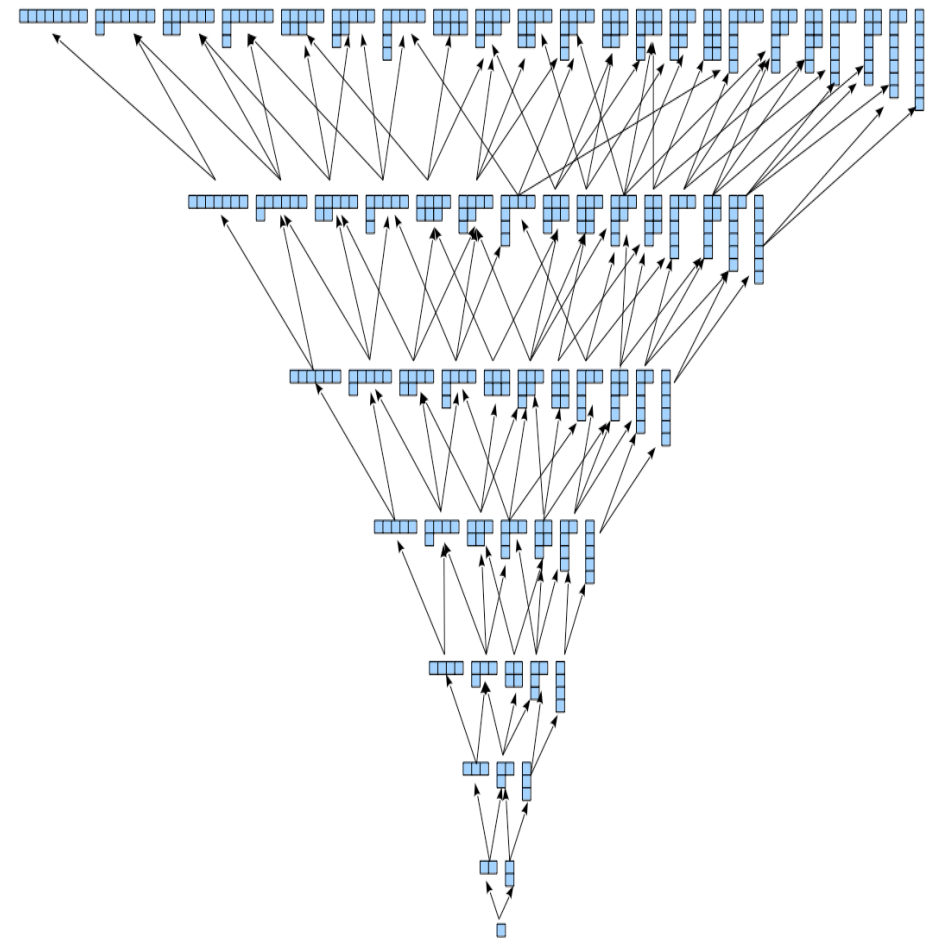
\includegraphics[scale=0.45]{Pictures/youngslattice.png}
                \caption{Young's lattice.}
            \end{figure}

            Young's lattice possess the folling symmetry: the partition $n+n-1+\dots2+1$ of the $n$th triangular number has a Young diagram that looks like a staircase. If we now only keep the elements whose hull is contained in this staircase, we get a subset of Young's lattice. When rank-embedded, this subset clearly has the expected bilateral symmetry of Young's lattice but also a rotational symmetry, which appear more clearly if we move away from this rank-embedding. The rotation group of order $n+1$ acts on this poset\footnote{Partially ordered set.}. Since it has both a bilateral and a rotational symmetry it must also have a dihedral symmetry and, indeed, the dihedral group $\D_{n+1}$ acts faithfully on this set.

            \begin{figure}[H]
                \centering
                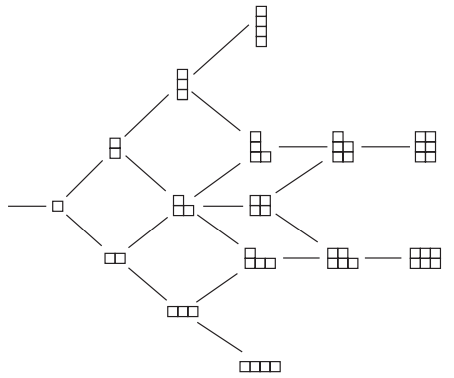
\includegraphics[scale=0.45]{Pictures/suter1.png}
                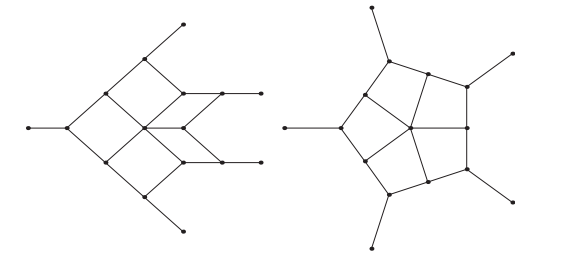
\includegraphics[scale=0.45]{Pictures/suter2.png}
                \caption{Example of dihedral symmetry for $n=4$.}
            \end{figure}

\section{Some derivations}

    \subsection{Invariant configurations for $\C\times\C^2/2\D_n$}\label{app:invconfDn}

        \subsubsection{Gauge field}

            To find the invariant configurations of the gauge group, we use use the bi-index notation and split the sub-blocks of $A_\mu$ in four categories depending on the dimensionality of the representations that they transform in. Note that it is only necessary to check the invariance under the two generators of $2\D_n$ to ensure invariance under the whole group.
            \begin{itemize}
                \item components $A_{\mu;a\alpha_a,b\beta_b}$ are $1\times 1$ blocks that transform as $A_{\mu;a\alpha_a,b\beta_b}\mapsto\sigma_a(\gamma)A_{\mu;a\alpha_a,b\beta_b}\sigma_b(\gamma)^{-1}$. It follows that only the component with $a,b=0,1$ or $a,b=2,3$ can be non-zero to have invariance under $A$. For invariance under $B$, we find that only the component with $a,b=0,2$ or $a,b=1,3$ can be non-zero if $n$ is even and only the component with $a=b$ if $n$ is odd. In conclusion, the invarint configuration under $A$ and $B$ are of the form
                \begin{equation}
                    (A_{\mu;ab})=\begin{bmatrix}
                        \times & 0 & 0 & 0 \\
                        0 & \times & 0 & 0 \\
                        0 & 0 & \times & 0 \\
                        0 & 0 & 0 & \times
                    \end{bmatrix}
                \end{equation}
                regardless of the parity of $n$.
                \item components $A_{\mu;a\alpha_a,r\beta_r}$ are $1\times 2$ blocks that transform as $A_{\mu;a\alpha_a,r\beta_r}\mapsto\sigma_a(\gamma)A_{\mu;a\alpha_a,r\beta_r}\mu_r(\gamma)^{-1}$. More explicitely, each block is of the form $\begin{bmatrix} x_1 & x_2 \end{bmatrix}$ and transforms as
                \begin{equation*}
                    \begin{bmatrix} x_1 & x_2 \end{bmatrix}\mapsto\sigma_a(A)\begin{bmatrix} x_1\zeta^{-r}_{2n} & x_2\zeta^{r}_{2n} \end{bmatrix}
                \end{equation*}
                under the generator $A$. This never invariant unless $a=b=0$. There is no need to check the invariance under $B$ since all these component are already all zero.
                \item components $A_{\mu;r\alpha_r,a\beta_a}$ are $2\times 1$. The situation is exactly the samme as in the previous point: they must all vanish.
                \item components $A_{\mu;r\alpha_r,s\beta_s}$ are $2\times 2$ blocks that transform as $A_{\mu;r\alpha_r,s\beta_s}\mapsto\mu_r(\gamma)A_{\mu;r\alpha_r,s\beta_s}\mu_s(\gamma)^{-1}$. Generically speaking, an invariant block under $A$ must satisfy
                \begin{equation}
                    \begin{bmatrix}
                        \zeta^{r}_{2n} & 0 \\
                        0 & \zeta^{-r}_{2n}
                    \end{bmatrix}
                    \begin{bmatrix}
                        x_1 & x_2 \\
                        x_3 & x_4
                    \end{bmatrix}
                    \begin{bmatrix}
                        \zeta^{-s}_{2n} & 0 \\
                        0 & \zeta^{s}_{2n}
                    \end{bmatrix}=
                    \begin{bmatrix}
                        x_1\zeta^{r-s}_{2n} & x_2\zeta^{r+s}_{2n} \\
                        x_3\zeta^{-r-s}_{2n} & x_4\zeta^{-r+s}_{2n}
                    \end{bmatrix}=
                    \begin{bmatrix}
                        x_1 & x_2 \\
                        x_3 & x_4
                    \end{bmatrix}.
                \end{equation}
                There are two possibilities to have non-vanishing component: $\zeta^{r-s}_{2n}=1$ and $x_2=x_3=0$ or $\zeta^{r+s}_{2n}=1$ and $x_1=x_4=0$ but the latter is actually not possible since $r,s=1,\dots,n-1$. To we find that the blocks must be of the form
                \begin{equation}
                    A_{\mu;r\alpha_r,s\beta_s}=
                        \begin{bmatrix}
                            \times & 0 \\
                            0 & \times
                        \end{bmatrix}
                \end{equation}
                if $r=s$ and vanishing otherwise. For invariance under $B$, a blocks must satisfy
                \begin{equation}
                    \begin{bmatrix}
                        0 & -1 \\
                        1 & 0
                    \end{bmatrix}
                    \begin{bmatrix}
                        x_1 & x_2 \\
                        x_3 & x_4
                    \end{bmatrix}
                    \begin{bmatrix}
                        0 & -1 \\
                        1 & 0
                    \end{bmatrix}=
                    \begin{bmatrix}
                        -x_4 & x_3 \\
                        x_2 & -x_1
                    \end{bmatrix}=
                    \begin{bmatrix}
                        x_1 & x_2 \\
                        x_3 & x_4
                    \end{bmatrix}.
                \end{equation}
                which is only possible if $x_1-x_4$ and $x_2=x_3$. Finally, we find that invariance under $A$ and $B$ imposes the block to be of the form
                \begin{equation}
                    A_{\mu;r\alpha_r,s\beta_s}=
                        \begin{bmatrix}
                            x & 0 \\
                            0 & -x
                        \end{bmatrix}
                \end{equation}
                if $r=s$ and vanishing otherwise.
            \end{itemize}
            The invariant gauge field configurations were found to be of the form
            \begin{equation}
                A_\mu=
                {\tiny
                \left[
                \begin{array}{*{20}c}
                    \times & 0 & 0 & 0 & & & & & & \cdots & 0 \\
                    0 & \times & 0 & 0 & & & & & & & \\
                    0 & 0 & \times & 0 & & & & & & & \\
                    0 & 0 & 0 & \times & & & & & & & \\
                    & & & & x_1 & 0 & & & & & \\
                    & & & & 0 & -x_1 & & & & & \\
                    & & & & & & x_2 & 0 & & & \\
                    & & & & & & 0 & -x_2 & & & \\
                    \vdots & & & & & & & & \ddots & & \vdots \\
                    & & & & & & & & & x_{n-1} & 0 \\
                    0 & & & & & & & & & 0 & -x_{n-1}
            \end{array}
            \right]}\label{eq:invformAmuDn}
            \end{equation}
            where each entry $(i,j)$ is an arbitrary block of size $N_i\times N_j$.

        \subsubsection*{Scalar fields}

            For the real scalar fields $X^m$, we need the action of $2\D_n$ on $\C^3$:
            \begin{equation}
                \begin{bmatrix}
                    z_1\\z_2\\z_3
                \end{bmatrix}\overset{A}{\longmapsto}
                \begin{bmatrix}
                    1 & 0 & 0 \\
                    0 & \zeta_{2n} & 0 \\
                    0 & 0 & \zeta^{-1}_{2n}
                \end{bmatrix}
                \begin{bmatrix}
                    z_1\\z_2\\z_3
                \end{bmatrix},\qquad
                \begin{bmatrix}
                    z_1\\z_2\\z_3
                \end{bmatrix}\overset{B}{\longmapsto}
                \begin{bmatrix}
                    1 & 0 & 0 \\
                    0 & 0 & i \\
                    0 & i & 0
                \end{bmatrix}
                \begin{bmatrix}
                    z_1\\z_2\\z_3
                \end{bmatrix}.\label{eq:RsymDn}
            \end{equation}
            The partitionning of $X^m$ is similar to $A_\mu$. The additional difficulty is come from R-symmetry. Since it acts differently on the different components, we have the study themalmost one by one.
            \begin{itemize}
                \item the fields $X^0$ and $X^1$ are left untouched by R-symmetry, meaning that the invariant configurations have the same form than the gauge field, i.e. \eqref{eq:invformAmuDn}.
                \item $X^{2,3}_{a\alpha_a,b\beta_b}$ transforms under $A$ as $X^{2,3}_{a\alpha_a,b\beta_b}\mapsto \xi_{2n}\sigma_a(A) X^{2,3}_{a\alpha_a,b\beta_b}\sigma_b(A)^{-1}$. The only configurations that are left invariant are therefore the ones such that $ \xi_{2n}\sigma_a(A) \sigma_b(A)^{-1}=1$, which is never the case. So $X^{2,3}_{a\alpha_a,b\beta_b}=0$ for all $a,b=0,\dots,3$.
                \item $X^{2,3}_{a\alpha_a,k\beta_k}$ transforms under $A$ as $X^{2,3}_{a\alpha_a,k\beta_k}\mapsto \xi_{2n}\sigma_a(A) X^{2,3}_{a\alpha_a,k\beta_k}\mu_k(A)^{-1}$. More explicitely, if we denote a block$X^{2,3}_{a\alpha_a,k\beta_k}$ by $\begin{bmatrix} x_1 & x_2 \end{bmatrix}$, we get
                \begin{equation}
                    \begin{bmatrix}
                        \xi^{k+1}_{2n}\sigma_a(A) x_1 & \xi^{-k+1}_{2n}\sigma_a(A) x_2
                    \end{bmatrix}=
                    \begin{bmatrix}
                        x_1 & x_2
                    \end{bmatrix}
                \end{equation}
                therefore we can have $x_1\neq0$ iff $\sigma_a(A)=-1$(i.e. $a=2,3$) and $k=n-1$, and we can have $x_1\neq0$ iff $\sigma_a(A)=1$(i.e. $a=0,1$) and $k=1$.
                \item $X^{2,3}_{k\alpha_k,b\beta_b}$ transforms under $A$ as $X^{2,3}_{k\alpha_k,b\beta_b}\mapsto \xi_{2n}\mu_k(A) X^{2,3}_{k\alpha_k,b\beta_b}\sigma_a(A)^{-1}$. Similarly to the previous case, we can write the blocks $X^{2,3}_{k\alpha_k,a\beta_a}$ as $\begin{bmatrix} x_1 \\ x_2 \end{bmatrix}$, we get
                \begin{equation}
                    \begin{bmatrix}
                        \xi^{k+1}_{2n}\sigma_a(A) x_1 \\ \xi^{-k+1}_{2n}\sigma_a(A) x_2
                    \end{bmatrix}=
                    \begin{bmatrix}
                        x_1 \\ x_2
                    \end{bmatrix}
                \end{equation}
                therefore the conditions are exactly the same: we can have $x_1\neq0$ iff $\sigma_a(A)=-1$(i.e. $a=2,3$) and $k=n-1$, and we can have $x_1\neq0$ iff $\sigma_a(A)=1$(i.e. $a=0,1$) and $k=1$.
                \item $X^{2,3}_{k\alpha_k,l\beta_l}$ transforms under $A$ as $X^{2,3}_{k\alpha_k,l\beta_l}\mapsto \xi_{2n}\mu_k(A) X^{2,3}_{k\alpha_k,l\beta_l}\mu_l(A)^{-1}$. Again, we can write the blocks $X^{2,3}_{k\alpha_k,l\beta_l}$ as $\begin{bmatrix} x_1 & x_2 \\ x_3 & x_4 \end{bmatrix}$ and we get
                \begin{equation}
                    \begin{bmatrix} 
                        \zeta^{k-l+1}_{2n}x_1 & \zeta^{k+l+1}_{2n}x_2 \\
                        \zeta^{-k-l+1}_{2n}x_3 & \zeta^{-k+l+1}_{2n}x_4 
                    \end{bmatrix}=
                    \begin{bmatrix} 
                        x_1 & x_2 \\
                        x_3 & x_4 
                    \end{bmatrix}
                \end{equation}
                therefore, we can have
                \begin{itemize}
                    \item $x_1\neq0$ iff $l=k+1$,
                    \item $x_2\neq0$ iff $l=-k-1$ (not possible),
                    \item $x_3\neq0$ iff $l=-k+1$ (not possible),
                    \item $x_4\neq0$ iff $l=k-1$.
                \end{itemize}
                For $X^{4,5}_{i\alpha_i,j\beta_j}$, the reasonning is exactly the same but with the $R$-symmetry acting as $\zeta^{-1}_{2n}$ instead of $\zeta_{2n}$. After similar computations, we get that the components $X^{4,5}_{a\alpha_a,b\beta_b}$ must be all vanishing too and the components $X^{4,5}_{a\alpha_a,k\beta_k} = \begin{bmatrix} x_1 & x_2 \end{bmatrix}$ can have $x_1\neq0$ iff $a=0,1$ and $k=1$ and $x_2\neq0$ iff $a=2,3$ and $k=n-1$. The same goes for the components $X^{4,5}_{k\alpha_k,b\beta_b}=\begin{bmatrix}x_1\\ x_2\end{bmatrix}$ and, at last, for the components $X^{4,5}_{k\alpha_k,l\beta_l}=\begin{bmatrix} 
                    x_1 & x_2 \\
                    x_3 & x_4 
                \end{bmatrix}$, we find 
                \begin{itemize}
                    \item $x_1\neq0$ iff $l=k-1$,
                    \item $x_2\neq0$ iff $l=-k+1$ (not possible),
                    \item $x_3\neq0$ iff $l=-k-1$ (not possible),
                    \item $x_4\neq0$ iff $l=k+1$.
                \end{itemize}
            \end{itemize}

            We have established what configurations are invariant under the generator $A$, equivalently under the subgroup of $2\D_n$ generated by $A$. What about $B$? The action of $R$-symmetry for $B$ is more tiresome because it is not diagonal, see \eqref{eq:RsymDn}.  This implies that components get exchanged. More precisely, recall our notations $z_1=X^0+iX^1$, etc, if we rewrite \eqref{eq:RsymDn} in terms of real components, we get that
            \begin{equation}
                \begin{bmatrix}
                    X^0\\X^1\\X^2\\X^3\\X^4\\X^5
                \end{bmatrix}\overset{B}{\longmapsto}
                \begin{bmatrix}
                    X^0\\X^1\\-X^5\\X^4\\-X^3\\X^2
                \end{bmatrix}.
            \end{equation}
            For the components $X^2_{a\alpha_a,b\beta_b}$, this implies that $X^2_{a\alpha_a,b\beta_b}=-\sigma_a(B)\sigma_b(B)^{-1}X^5_{a\alpha_a,b\beta_b}$. This completely fixes $X^5_{a\alpha_a,b\beta_b}$ in terms of $X^2_{a\alpha_a,b\beta_b}$. The can be done the other components of $X^2$, they we find that they all determine the ones of $X^5$. Without fully splitting each fields into components, we see that we must have
            \begin{align}
                X^2_{ij}&=-\rho_i(B)X^5_{ij}\rho_j(B)^{-1},\\
                X^3_{ij}&=\rho_i(B)X^4_{ij}\rho_j(B)^{-1},\\
                X^4_{ij}&=-\rho_i(B)X^3_{ij}\rho_j(B)^{-1},\\
                X^5_{ij}&=\rho_i(B)X^2_{ij}\rho_j(B)^{-1},\\
            \end{align}
            bto have invariance under $B$. This equations imply in particular that $X^2_{kl}=-\rho_k(B^2)X^2_{kl}\rho_l(B^2)^{-1}$. Since, $\rho_k(B^2)=-\mathbbm{1}_{2\times 2}$ for every $k$, we get that all components $X^2_{kl}$ must be vanishing. In turn, this implies the components $X^{3,4,5}_{kl}$ must also all vanish. \todo{This cannot be true.}


    \subsection{}\label{app:compsum}

        We want to compute the sum
        \begin{equation}
            \sum^{\lfloor n/3\rfloor}_{a=1}~\left\lfloor \frac{n-3a}{2}+1\right\rfloor = \left\lfloor \frac{n}{3}\right\rfloor + \sum^{\lfloor n/3\rfloor}_{a=1}~\left\lfloor \frac{n-3a}{2}\right\rfloor.
        \end{equation}
        Let us write $n\in\N$ as $n=3m+r$ with $r=0,1$ or $2$ and $m\in\N$. Regardless of $r$, we have $\lfloor n/3\rfloor=m$ and
        \begin{equation}
            \sum^{\lfloor n/3\rfloor}_{a=1}~\left\lfloor \frac{n-3a}{2}\right\rfloor = \sum^{m}_{a=1}~\left\lfloor \frac{3}{2}(m-a)+\frac{r}{2}\right\rfloor = \sum^{m-1}_{a=0}~\left\lfloor \frac{3}{2}a+\frac{r}{2}\right\rfloor.\label{eq:sumfloor}
        \end{equation}
        \begin{itemize}
            \item if $r=0$, then \eqref{eq:sumfloor} becomes
            \begin{equation}
                \sum^{m-1}_{a=0}~\left\lfloor \frac{3}{2}a\right\rfloor = \sum^{m-1}_{a=0}~a+\sum^{m-1}_{a=0}~\left\lfloor \frac{a}{2}\right\rfloor = \frac{(m-1)m}{2}+\sum^{m-1}_{a=0}~\left\lfloor \frac{a}{2}\right\rfloor.
            \end{equation}
            Now if $m$ is even, we have
            \begin{equation}
                \sum^{m-1}_{a=0}~\left\lfloor \frac{a}{2}\right\rfloor = 2\sum^{\left\lfloor \frac{m-1}{2}\right\rfloor}_{a=0}~a = 2\sum^{\frac{m}{2}-1}_{a=0}~a = \left(\frac{m}{2}-1\right)\frac{m}{2}
            \end{equation}
            and if $m$ is odd,
            \begin{equation}
                \sum^{m-1}_{a=0}~\left\lfloor \frac{a}{2}\right\rfloor = 2\sum^{\left\lfloor \frac{m-2}{2}\right\rfloor}_{a=0}~a+\left\lfloor \frac{m-1}{2}\right\rfloor = 2\sum^{ \frac{m-3}{2}}_{a=0}~a+\frac{m-1}{2} = \frac{(m-1)^2}{4}
            \end{equation}
            so
            \begin{equation}
                \sum^{m-1}_{a=0}~\left\lfloor \frac{a}{2}\right\rfloor = 
                \begin{cases}
                    \left(\frac{m}{2}-1\right)\frac{m}{2},\qquad\text{if $m$ is even}\\
                    \frac{(m-1)^2}{4},\qquad\text{if $m$ is odd}
                \end{cases}.\label{eq:suma2floor}
            \end{equation}
            and
            \begin{equation}
                \sum^{m-1}_{a=0}~\left\lfloor \frac{3a}{2}\right\rfloor = 
                \begin{cases}
                    \frac{m(3m-4)}{4},\qquad\text{if $m$ is even}\\
                    \frac{(m-1)(3m-1)}{4},\qquad\text{if $m$ is odd}
                \end{cases}.\label{eq:sum3a2floor}
            \end{equation}
            \item if $r=1$, then \eqref{eq:sumfloor} becomes
            \begin{equation}
                \sum^{m-1}_{a=0}~\left\lfloor \frac{3}{2}a+\frac{1}{2}\right\rfloor = \sum^{m-1}_{a=0}~a+\sum^{m-1}_{a=0}~\left\lfloor \frac{a+1}{2}\right\rfloor = \frac{(m-1)m}{2}+\sum^{m-1}_{a=0}~\left\lfloor \frac{a+1}{2}\right\rfloor
            \end{equation}
            and
            \begin{equation}
                \sum^{m-1}_{a=0}~\left\lfloor \frac{a+1}{2}\right\rfloor = \sum^{m}_{a=1}~\left\lfloor \frac{a}{2}\right\rfloor = \sum^{m}_{a=0}~\left\lfloor \frac{a}{2}\right\rfloor =  
                \begin{cases}
                    \frac{m^2}{4},\qquad\text{if $m$ is even}\\
                    \frac{m^2-1}{4},\qquad\text{if $m$ is odd}
                \end{cases}
            \end{equation}
            by \eqref{eq:suma2floor} so
            \begin{equation}
                \sum^{m-1}_{a=0}~\left\lfloor \frac{3}{2}a+\frac{1}{2}\right\rfloor=
                \begin{cases}
                    \frac{m(3m-2)}{4},\qquad\text{if $m$ is even}\\
                    \frac{3m^2-2m-1}{4},\qquad\text{if $m$ is odd}
                \end{cases}
            \end{equation}
            \item if $r=2$, then \eqref{eq:sumfloor} becomes
            \begin{equation}
                \sum^{m-1}_{a=0}~\left\lfloor \frac{3}{2}a+1\right\rfloor = m+\sum^{m-1}_{a=0}~\left\lfloor \frac{3}{2}a\right\rfloor.
            \end{equation}
            so
            \begin{equation}
                \sum^{m-1}_{a=0}~\left\lfloor \frac{3}{2}a+1\right\rfloor=
                \begin{cases}
                    \frac{3m^2}{4},\qquad\text{if $m$ is even}\\
                    \frac{3m^2+1}{4},\qquad\text{if $m$ is odd}
                \end{cases}
            \end{equation}
            from \eqref{eq:sum3a2floor}.
        \end{itemize}
        Finally, we can write $m=2k$ if $m$ if even and $m=2k+1$ if $m$ is odd in order to distinguish the six different cases. We get
        \begin{align}
            a(n)\equiv\sum^{\lfloor n/3\rfloor}_{a=1}~\left\lfloor \frac{n-3a}{2}+1\right\rfloor&=
            \begin{cases}
                2k+\frac{2k(6k-4)}{4},\qquad\text{if $n=6k$}\\
                2k+\frac{2k(6k-2)}{4},\qquad\text{if $n=6k+1$},\\
                2k+\frac{12k^2}{4},\qquad\text{if $n=6k+2$},\\
                (2k+1)+\frac{2k(6k+2)}{4},\qquad\text{if $n=6k+3$},\\
                (2k+1)+\frac{3(2k+1)^2-2(2k+1)-1}{4},\qquad\text{if $n=6k+4$},\\
                (2k+1)+\frac{3(2k+1)^2+1}{4},\qquad\text{if $n=6k+5$}
            \end{cases}\\
            &=
            \begin{cases}
                3k^2,\qquad\text{if $n=6k$}\\
                3k^2+k,\qquad\text{if $n=6k+1$},\\
                3k^2+2k,\qquad\text{if $n=6k+2$},\\
                3k^2+3k+1,\qquad\text{if $n=6k+3$},\\
                3k^2+4k+1,\qquad\text{if $n=6k+4$},\\
                3k^2+5k+2,\qquad\text{if $n=6k+5$}
            \end{cases}.
        \end{align}
        Starting from $n=1$, the first value of this sequence is : $0,0,1,1,2,3,4,5,7,8,10,12,\dots$. Uppon  further analysis, this correspond to the sequence \href{https://oeis.org/A001399}{\textcolor{blue}{\underline{A001399}}}, that have several interpretations:
        \begin{itemize}
            \item the number of partitions of $n$ into at most 3 parts. This makes sense with our initial problem: finding all the $a,b,c$'s such that $a+b+c=n$,
            \item the number of connected graphs with $3$ nodes and $n$ edges (where multiple edges between the same nodes are allowed),
            \item the number of non-negative solutions to $b+2c+3d=n$,
        \end{itemize}
        as well as many others. Finally, we note that we can simply write
        \begin{equation}
            a(n)=\text{round}\left(\frac{n^2}{12}\right).
        \end{equation}

\section{References guide}

    \begin{itemize}
        \item General strings and D-branes: \cite{DbranespartI},\cite{DbranespartII},\cite{notesDbranes}
        \item He: review: \cite{he2004lectures}, thesis: \cite{masterHe}
        \item Orbifold construction for $\Gamma\subset\SU(2)$: type $A$ : \cite{douglas1996dbranes}, type $D$ and $E$: \cite{PhysRevD.55.6382}
        \item Orbifold construction for $\Gamma\subset\SU(3)$:\cite{Hanany_1999}
        \item Orbifold construction for $\Gamma\subset\SU(4)$:\cite{Hanany:1999sp}
        \item Formalization of projection to daughter theories: \cite{vafa1998},\cite{silervstein1998}
        \item Quivers representations and varieties: \cite{brion},\cite{kirillov2016quiver}
        \item On toric varieties: \cite{cox2011toric},\cite{torigeomandCY}(\cite{fulton1993introduction},\cite{oda1988convex})
        \item Forward algorithm  for toric singularities devlopments: \cite{FA1},\cite{FA2},\cite{FA3},\cite{FA4},\cite{FA5}, formalization: \cite{FA6},\cite{FA7},\cite{FA8}
        \item Toric diagrams, dimer diagrams and Higgsing: \cite{Argurio_20081}
        \item Fractional branes: \cite{Argurio_20082}
        \item Formalization of inverse algorithm for toric singularities: \cite{Feng_2001}
        \item geometry and K3 surfaces: \cite{https://doi.org/10.48550/arxiv.hep-th/9611137}
        \item general review of SYM and their brane description: \cite{Elitzur_1997}
        \item Hanany-Witten setup: \cite{1997}
        \item geometric engineering: \cite{https://doi.org/10.48550/arxiv.hep-th/9706110},\cite{Katz:1996xe},\cite{Katz:1996fh}
        \item link between graph theory and Yang-Mills (constructed from string theory with the three different methods) to study the finiteness of the theories: \cite{Hanany:1999sp}
    \end{itemize}

\section{References guide}

\begin{itemize}
    \item He: review: \cite{he2004lectures}, thesis: \cite{masterHe}
    \item Orbifold construction for $\Gamma\subset\SU(2)$: type $A$ : \cite{douglas1996dbranes}, type $D$ and $E$: \cite{PhysRevD.55.6382}
    \item Orbifold construction for $\Gamma\subset\SU(3)$:\cite{Hanany_1999}
    \item Formalization of projection to daughter theories: \cite{vafa1998},\cite{silervstein1998}
    \item On toric varieties: \cite{cox2011toric},\cite{torigeomandCY}(\cite{fulton1993introduction},\cite{oda1988convex})
    \item Forward algorithm  for toric singularities: devlopments: \cite{FA1},\cite{FA2},\cite{FA3},\cite{FA4},\cite{FA5}, formalization: \cite{FA6},\cite{FA7},\cite{FA8}
    \item Toric diagrams, dimer diagrams and Higgsing: \cite{Argurio_20081}
    \item Fractional branes: \cite{Argurio_20082}
    \item Quiver representations and quiver varities: \cite{kirillov2016quiver}
    \item Formalization of inverse algorithm for toric singularities: \cite{Feng_2001}
\end{itemize}

The bests:
\begin{itemize}
    \item \cite{bertolinisusy}
    \item \cite{DbranespartI,DbranespartII}
    \item \cite{he2004lectures}
    \item \cite{brion}
    \item \cite{torigeomandCY}
\end{itemize}

\pagebreak

\listofmarker
\addcontentsline{toc}{section}{\listmarkername}

\pagebreak

\printbibliography

\end{document}